\documentclass[12pt,a4paper]{report}

% Packages
\usepackage[margin=1in]{geometry}
\usepackage{graphicx}
\usepackage{titlesec, blindtext, color, float}
\usepackage{hyperref}
\usepackage{setspace}
\usepackage{enumitem}
\usepackage{mdframed}
\usepackage{pdflscape}
\usepackage{lipsum}
\usepackage{tabularx}
\usepackage{multirow}
\usepackage{array}
\usepackage{makecell}
\usepackage{longtable}




\titleformat
  {\chapter}              % command
  [display]               % shape
  {\centering\bfseries\Huge}        % format applied to label and title
  {Chapter \thechapter}   % label
  {0pt}                   % sep (zero separation)
  {% before-code: top rule, then center immediately
    \centering
  }

\titlespacing*{\chapter}
{0pt}    % left
{0pt}    % space before title
{20pt}   % space after title

\titlespacing*{\section}{0pt}{2ex}{1ex}
\titlespacing*{\subsection}{0pt}{2ex}{1ex}
  
\begin{document}
% Title Info
\pagenumbering{gobble}
\begin{center}
	\textbf{\Huge{DeepFake detection using Deep Learning}}\\[2em]

\Large {{\textbf{A Project Report }}}\\[1em]
\large \textit{\textbf{Submitted by }}\\[1em]

\Large\textbf{{\centering{Kaibalya Prasad Nayak (Reg. No: 2241014084 )\\
                  Rupali Bisoyi (Reg. No: 2241002192 )\\
                  Saswat Kumar Nayak (Reg. No: 2241014125 )\\
                  Sameera Kar (Reg. No: 2241011022 )\\[2em]}}}
\centering{in partial fulfillment for the award of the degree of} \\[1em]
\Large\textbf{{BACHELOR OF TECHNOLOGY  \\ IN \\COMPUTER SCIENCE \& ENGINEERINNG}}\\
(Specialization in Artificial Intelligence and Machine Learning)




                  
\vspace*{\fill}
                  

\includegraphics[scale=0.2]{one.png} 

\vspace*{\fill}
\large \textbf {Centre for Artificial Intelligence and Machine Learning} \\
\Large \textbf {Department of Computer Science and Engineering} \\
\large \textbf{Faculty of Engineering and Technology} \\ Institute of Technical Education and Research
\\
\LARGE \textbf{Siksha `O' Anusandhan \\(Deemed to be University)}\\
\large Bhubaneswar, Odisha, India\\
\large \textbf{June, 2026}
\end{center}


\setstretch{1.5}

\chapter*{CERTIFICATE}
\begin{center}
	
\includegraphics[scale=0.2]{one.png}
\end{center} 

\noindent This is to certify that the project report titled “\textbf{DeepFake detection using Deep Learning}” being submitted by \textbf{Kaibalya Prasad Nayak, Rupali Bisoyi, Saswat Kumar Nayak, Sameera Kar} of \textbf{Section - 32} to the \textbf{Institute of Technical Education and Research, Siksha ‘O’ Anusandhan (Deemed to be University) }, Bhubaneswar for the partial fulfillment for the degree of \textbf{Bachelor of Technology in Computer Science and Engineering (Specialization in Artificial Intelligence and Machine Learning)} is a record of original confide work carried out by them under our supervision and guidance. The project work, in my opinion, has reached the requisite standard fulfilling the requirements for the Degree of \textbf{Bachelor of Technology}. 

\noindent The results contained in this project work have not been submitted in part or full to any other University or Institute for the award of any degree or diploma.

\vfill{}

\noindent\begin{tabular}{p{15cm} p{0.0cm}}
\rule{6.2cm}{0.5pt} & \\
\textbf{Mr.Abdul Atif Khan} &\\
Assistant professor &\\
Centre for Artificial Intelligence and Machine Learning &\\
Department of Computer Science \& Engineering &\\
Faculty of Engineering \& Technology, Institute of Technical Education and Research &\\
\textbf{Siksha `O' Anusandhan (Deemed to be University),  Bhubaneswar}
&\\

\end{tabular}


\chapter*{ACKNOWLEDGEMENT}
We would like to express our sincere gratitude to our guide, \textbf{Mr.\ Abdul Atif Khan}, Centre for Artificial Intelligence and Machine Learning, ITER, Siksha `O' Anusandhan University, for his valuable guidance, continuous support, and encouragement throughout the completion of this project work. We are also thankful to the faculty members of the Centre for Artificial Intelligence and Machine Learning for providing us with the necessary resources and technical support required for this research work. We express our heartfelt gratitude to our parents, friends, and well-wishers for their constant motivation and encouragement throughout the project. Finally, we would like to thank Siksha `O' Anusandhan University for providing us with the opportunity and infrastructure to carry out this research successfully.
\vfill
\begin{center}
\begin{tabular}{p{5.2cm}p{5.8cm}p{3.2cm}}
\textbf{Name of Student} & \textbf{Roll No.} & \textbf{Signature} \\[1em]
Kaibalya Prasad Nayak & Reg. No. 2241014084& \rule{3.2cm}{0.2pt} \\[1em]
Rupali Bisoyi & Reg. No. 2241002192& \rule{3.2cm}{0.2pt} \\[1em]
Saswat Kumar Nayak & Reg. No. 2241014125& \rule{3.2cm}{0.2pt} \\[1em]
Sameera Kar & Reg. No. 2241011022& \rule{3.2cm}{0.2pt} \\[1em]
\end{tabular}
\end{center}
\vspace{1cm}
\noindent\textbf{Date:} \rule{5cm}{0.2pt} \hfill \textbf{Place:} \rule{5cm}{0.2pt}


\chapter*{DECLARATION}
We declare that this written submission represents our ideas in our own words and where other’s ideas or words have been included, we have adequately cited and referenced the original sources. We also declare that we have adhered to all principles of academic honesty and integrity and have not misrepresented or fabricated or falsified any idea/fact/source in our submission. We understand that any violation of 
the above will cause for disciplinary action by the University and can also evoke penal action from the sources which have not been properly cited or from whom proper permission has not been taken when needed.
\vspace{1cm}

\begin{center}
\begin{tabular}{p{5.2cm}p{5.8cm}p{3.2cm}}
\textbf{Name of Student} & \textbf{Roll No.} & \textbf{Signature} \\[1em]
Kaibalya Prasad Nayak & Reg. No. 2241014084& \rule{3.2cm}{0.2pt} \\[1em]
Rupali Bisoyi & Reg. No. 2241002192& \rule{3.2cm}{0.2pt} \\[1em]
Saswat Kumar Nayak & Reg. No. 2241014125& \rule{3.2cm}{0.2pt} \\[1em]
Sameera Kar & Reg. No. 2241011022& \rule{3.2cm}{0.2pt} \\[1em]
\end{tabular}
\end{center}
\vspace{1cm}
\noindent\textbf{Date:} \rule{5cm}{0.2pt} \hfill \textbf{Place:} \rule{5cm}{0.2pt}



\chapter*{REPORT APPROVAL}

This project report titled “\textbf{DeepFake detection using Deep Learning}” submitted by  \textbf{Kaibalya Prasad Nayak, Rupali Bisoyi, Saswat Kumar Nayak, Sameera Kar} is approved for the degree of \textbf{Bachelor of Technology} in \textbf{Computer Science and Engineering (Specialization in Artificial Intelligence and Machine Learning)}.

\vspace{2cm}
\noindent\begin{tabular}{p{9cm} p{7cm}}
\textbf{Examiner(s)} &\\[0.75cm]
\rule{6.2cm}{1pt} & \\[0.75cm]
\rule{6.2cm}{1pt} & \\[0.75cm]
\rule{6.2cm}{1pt} & \\[3cm]
\rule{6.2cm}{1pt} & \\
\textbf{Supervisor} &\\[3cm]
\rule{6.2cm}{1pt} & \rule{6.5cm}{1pt}\\
\textbf{Project Coordinator(s)} &\textbf{Chief Coordinator, CAIML}\\
\end{tabular}

\newpage
\chapter*{PREFACE}

Deepfake technology has emerged as one of the most transformative and consequential advancements in the domain of Artificial Intelligence and multimedia generation. Powered by sophisticated deep learning architectures such as Generative Adversarial Networks (GANs), Variational Autoencoders (VAEs), and diffusion-based models, deepfake systems are capable of producing hyper-realistic synthetic media that is increasingly indistinguishable from authentic content. Although such technologies offer several beneficial applications across entertainment, virtual reality, digital media production, film post-production, and accessibility services, their growing misuse has raised profound concerns regarding misinformation, identity theft, non-consensual content generation, cybercrime, and large-scale digital content manipulation. As synthetic media generation techniques continue to evolve at an unprecedented pace, the development of reliable, scalable, and automated deepfake detection systems has become not only a research imperative but also a societal necessity.

This project work presents a comprehensive deep learning-based framework for the detection of manipulated facial images and videos, leveraging the capabilities of EfficientNet B0 and a Hybrid CNN-Transformer architecture. The EfficientNet B0 model offers an optimal balance between accuracy and computational efficiency through its compound scaling strategy, while the Hybrid CNN-Transformer architecture combines the local feature extraction strengths of convolutional neural networks with the global contextual modeling power of transformer-based attention mechanisms. The proposed framework incorporates benchmark datasets, namely CelebDF-V2 and FaceForensics++, which represent diverse and challenging manipulation scenarios including face-swapping, expression transfer, and identity replacement. Robust facial region extraction is achieved using the Multi-Task Cascaded Convolutional Neural Network (MTCNN), which enables precise localization and alignment of facial landmarks prior to classification. A thorough comparative evaluation has been conducted to analyze and contrast the effectiveness, computational efficiency, generalization capability, and robustness of both architectures under varying conditions.


\newpage
\pagenumbering{roman}
\tableofcontents

\newpage
\addcontentsline{toc}{chapter}{LIST OF FIGURES}
\listoffigures

\newpage
\addcontentsline{toc}{chapter}{LIST OF TABLES}
\listoftables


\newpage
\pagenumbering{arabic} 
% ---------- Section 1 ----------
\chapter{INTRODUCTION}
\section{Introduction}

The technologies of generating multimedia have been transformed rapidly using Artificial Intelligence and Deep Learning. One of the most powerful and controversial of these advancements is the birth of deepfake technology. Deepfake technology has come to be one of the biggest and most interesting innovations among them. Deepfakes are synthetic media produced with the help of deep learning algorithms to manipulate the facial expression, voice or identity information featured in a photo or video in order to create a very realistic fake. At present, the major approaches for deepfake generation rely on Generative Adversarial Networks (GANs), autoencoders, and neural rendering techniques patel2026 [9],jheelan2025 [8]. While there are positive uses for deepfake technology in the movie industry, virtual reality and gaming, digital entertainment, and content creation, it has become a significant worldwide threat thanks to those malicious uses. Deepfake media can be used to disseminate misinformation, fake news, political propaganda, identity theft, financial fraud, cybercrime, and social engineering attacks pravallika2026 [1],ekatpure2025 [3]. As deepfake generation techniques continue to evolve, distinguishing manipulated media from authentic content becomes increasingly difficult. To compensate for these challenges, recently deep learning AI-based detection systems have received a lot of attention for their potential to detect and counter the presence of a deepfake. Convolutional Neural Networks (CNNs) and transformer-based architectures have demonstrated strong performance in extracting spatial and contextual features from manipulated facial regions bagherzadeh2023 [7],kosarkar2025 [10]. CNN models effectively capture low-level spatial inconsistencies, while transformer architectures improve contextual understanding and long-range dependency learning for robust deepfake detection. In this research work, a deep learning-based methodology for tackling classification of deepfake image/video forgeries is proposed. To provide comparative evaluations, the framework is based on EfficientNet\_B0 and Hybrid CNN-Transformer models. In the pre-processing stage, CelebDF-V2 and FaceForensics++ (FF-C23) are concatenated datasets, followed by facial feature extraction based on the MTCNN method where it involves MTCNN training with attention to strong facial representation learning.
\section{Project Overview / Problem Statement}
With the rapidly evolving technology of deepfakes that poses great question and challenge to verify and prove the real content behind anything digital, it is easy to view these as doctored images. The creation of deepfakes has come a long way and poses significant challenges to verifying the authenticity of digital content, and it is easy to see these as doctored images. GANs, autoencoders, and neural rendering techniques can create realistic facial photos and videos with genuine human-like features that are challenging for humans to tell apart from real media. The abuse of this Deep Fake technology has thus caused issues related to the spread of misinformation, of fake news, of the abuse of political apparatus, of identity theft, of cybercrime, financial crime, and privacy abuse. Traditional detection systems might fail to detect high-quality manipulations and have complexities, not to mention cross-dataset generalization issues. Another major challenge in deepfake detection is identifying manipulations in compressed and low-quality media. Compression algorithms often remove important forensic artifacts and facial inconsistencies that are useful for classification, making compressed deepfake detection significantly more difficult for existing deep learning systems. The need for an efficient and robust deepfake detection framework is great, because it should provide accurate detection of manipulated media with low computing requirements and a high generalization ability across several datasets.
\section{Motivations and Objectives}
\textbf{Motivations:} Generating deepfakes is now more attainable and common, driven largely by the increasing availability of AI technologies. Due to the increasing accessibility of deepfake creation tools, the production of synthetic media is becoming easier and more widespread. Manipulated media, which can be rapidly spread through social media platforms and digital communication systems, has raised the risks of misinformation and identity impersonation. Advanced deepfakes can be difficult to detect using traditional forensic techniques. This has driven progress in automated deep learning approaches capable of detecting subtle inconsistencies in manipulated facial content. In addition, with the development of CNN and Transformer architectures, more accurate and efficient deepfake detection models can be developed.

\textbf{Objectives:} The main goal of this research work is to develop a deep learning-based automated and unsupervised deepfake detection system for identifying manipulated facial images and videos that are difficult to detect visually. The proposed framework employs two specific deep learning architectures, namely EfficientNet\_B0 and a Hybrid CNN-Transformer, for deepfake classification, while MTCNN is used for facial feature extraction to enhance facial feature representation. This research also aims to merge the CelebDF-V2 and FaceForensics++ datasets for large-scale training and testing. Advanced preprocessing and data augmentation techniques are employed to improve model robustness and generalization ability. Moreover, the proposed models are evaluated using various performance measures such as accuracy, precision, recall, F1-score, confusion matrix analysis, and ROC-AUC score. The study further compares the EfficientNet\_B0 and Hybrid CNN-Transformer architectures to determine which architecture performs better for deepfake detection.
\section{Scope and Significance of the Work}
\textbf{Scope:} This research focuses on deep learning-based deepfake image and video detection. The proposed system is designed to detect manipulated facial content generated using advanced synthetic media technologies. The techniques involved include deepfake image and video classification, facial feature extraction using the MTCNN algorithm, and a comparative study of EfficientNet\_B0 and Hybrid CNN-Transformer models based on classification accuracy and computational efficiency. The proposed framework is trained and tested on benchmark datasets such as CelebDF-V2 and FaceForensics++. Implementation is carried out within a GPU-based deep learning environment to support large-scale experiments and efficient model training. The study focuses only on face-based deepfake detection and does not cover audio-only deepfake detection or multimodal forensic analysis.

\textbf{Significance:} Due to the rising use of synthetic media technologies and digital forgery, deepfake detection has become an important research field. The proposed framework helps mitigate risks associated with tampered digital content and enhances systems for verifying the authenticity of digital media. The significance of this research lies in improving cybersecurity and digital media verification through automated deepfake detection techniques. The framework can contribute toward reducing misinformation, fake news propagation, and manipulated content on the internet. It also enhances automated forensic analysis using deep learning architectures to detect manipulated facial images and videos. Furthermore, the proposed system provides a fast and accurate deepfake detection solution with improved generalization performance. The research also highlights the need for continued studies and innovations in AI-powered media forensics and deepfake detection technologies.

\section{Organisation of the Report}
The report is organized into several chapters, each focusing on a specific aspect of the research work.

Chapter 1 presents the introduction, problem statement, objectives, scope, significance, and motivation of the proposed work.

Chapter 2 discusses the literature review, existing deepfake detection methodologies, and identified research gaps.

Chapter 3 describes the materials and methods used in the proposed framework, including dataset descriptions, preprocessing techniques, system architecture, deep learning models, tools, technologies, and performance evaluation metrics.

Chapter 4 presents the experimental setup, implementation details, model configurations, and comparative analysis of the obtained results.

Chapter 5 discusses ethical considerations, societal impact, and sustainability aspects related to deepfake detection systems.

Chapter 6 summarizes the overall findings of the research work and discusses future enhancements and possible improvements in deepfake detection technologies.
\chapter{REVIEW OF LITERATURE}

Recently, there are several deep learning schemes proposed for deepfake detection, using architectures such as ResNeXt[6], hybrid CNN-LSTMs[7], and transfer learning approaches using MobileNetV2[8], which can effectively capture spatial and temporal artefacts and achieve high classification accuracy on benchmark datasets. However, existing frameworks suffer from critical limitations like limited generalisability across datasets, high computational complexity that limits their real-time deployment, and vulnerability to severe media compression. Moreover, traditional convolutional networks often do not have the contextual understanding needed to detect increasingly sophisticated high-quality GAN-generated fakes. To tackle these vulnerabilities and to minimise dataset bias, this research proposes a comparative deep learning framework with the use of EfficientNet\_B0 and Hybrid CNN-Transformer architectures. This work considers the optimal trade-off between computational efficiency and reliable contextual feature extraction for improved multimedia forensic analysis.
\section{Review of Existing Systems / Related Work}

Recent advancements in deep learning and computer vision have significantly improved the effectiveness of automated deepfake detection systems. Researchers have explored several approaches including CNN-based architectures, transformer models, transfer learning techniques, hybrid deep learning systems, and multimodal forensic frameworks for detecting manipulated media. Most existing research focuses on improving classification accuracy, computational efficiency, and robustness against sophisticated GAN-generated deepfake content. Benchmark datasets such as FaceForensics++ and CelebDF-V2 are widely used for evaluating the effectiveness of deepfake detection models. However, challenges such as poor cross-dataset generalization, compressed media detection, computational complexity, and robustness against high-quality synthetic media still remain unresolved.With the accelerated development of Artificial Intelligence (AI) technology and media generation techniques, deepfake detection has become a major research area. Several deep learning approaches have been proposed for detecting manipulated facial images, videos, and synthetic multimedia content. Pravallika and Tejaswini [3] developed a deep learning-based framework using ResNeXt architectures for detecting visual inconsistencies and temporal artifacts in manipulated media. Their work emphasized the importance of automated forensic systems for protecting the integrity of digital information and reducing the risks associated with synthetic media generation.Srinivasan et al. [6] proposed a Deepfake Detection Model (DDM) integrating Generative Adversarial Networks (GANs), Autoencoders, and Convolutional Neural Networks for real-time facial forgery detection. Their proposed system achieved an accuracy of approximately 92.3\% using custom celebrity datasets along with FaceForensics++, FakeAVCeleb, and DFFMD datasets.

Ekatpure et al. [7] introduced a deep learning framework combining CNN and hybrid LSTM architectures for deepfake image, video, and audio detection. Their methodology focused on automatic feature extraction instead of handcrafted forensic analysis and demonstrated the effectiveness of sequential deep learning models in identifying temporal manipulation patterns.
Deshpande et al. [8] proposed an automated CNN-based deepfake detection system for both images and videos. Their preprocessing pipeline included image resizing and transformation optimization, while the classification model achieved an accuracy of 95.775\%. The study demonstrated that optimized CNN architectures can effectively outperform traditional forensic approaches.Soppari et al.[9] presented a comprehensive survey on deepfake detection algorithms focusing on CNN- and EfficientNet-based architectures. Their work highlighted the role of feature extraction and deep learning-based classification in detecting subtle facial inconsistencies introduced during GAN-based media generation. Abhineswari et al. [10] conducted a comparative transfer learning study using multiple pretrained neural networks including MobileNetV2 and ResNet50 on the FaceForensics++ dataset. Their research demonstrated that MobileNetV2 achieved approximately 89\% accuracy and highlighted the effectiveness of transfer learning techniques in deepfake detection systems. Bagherzadeh and Rastgoo [4] proposed a hybrid deep convolutional neural network architecture combining multiple CNN models for enhanced feature extraction. 

Their approach improved classification robustness across diverse deepfake datasets containing more than 140,000 facial images. Jheelan and Pudaruth [2] investigated several pretrained deep learning models including MobileNet and InceptionV3 for detecting GAN-generated deepfakes. Their study achieved test accuracies as high as 98.5\% and emphasized the importance of preprocessing and face cropping for improving detection performance. Patel et al. [1] provided a comprehensive review of recent deepfake detection methodologies including CNNs, LSTMs, transformer-based systems, and multimodal architectures. Their work identified important research challenges such as dataset bias, computational complexity, and poor cross-dataset generalization. Kosarkar and Sakarkar [5] introduced a hybrid VARMA-LSTM-GRU architecture using dynamic spatio-temporal analysis for deepfake detection. Their system focused on identifying localized inconsistencies in motion and texture patterns while improving computational efficiency. Although previous studies achieved strong performance using CNNs, transfer learning, and hybrid sequential architectures, challenges such as computational complexity, dataset bias, limited robustness, and poor cross-dataset generalization still remain unresolved. Therefore, this research proposes a comparative framework using EfficientNet\_B0 and Hybrid CNN-Transformer architectures for robust and efficient deepfake detection.

\section{Research Gaps and Problem Identification}
The main limitation in the current deepfake detection literature is the ubiquitous use of intra-dataset evaluation protocols, which greatly hinders cross-dataset generalisation. Most existing models are trained, validated, and tested within a single isolated repository such as FaceForensics++ or CelebDF-V2. Consequently, these networks inadvertently overfit to the unique blending artefacts, specific illumination profiles, and proprietary compression algorithms inherent to a particular dataset. However, their classification accuracy drops drastically when challenged with unseen datasets or real-world multimedia content. This vulnerability exposes a fundamental flaw in domain adaptability and indicates the absence of reliable invariant feature extraction techniques capable of recognising the inherent statistical anomalies shared by all synthetic media rather than the digital signatures of a specific dataset.

In addition, while CNNs can effectively learn localised spatial features and high-frequency edge inconsistencies within facial patches, their local receptive fields are inherently incapable of modelling long-range global dependencies between different facial regions. This limitation is further exacerbated by the fact that few studies integrate a comprehensive set of diverse deepfake generation techniques such as FaceSwap, Face2Face, NeuralTextures, and FaceShifter into a unified training and evaluation pipeline. Existing frameworks, which are limited to specific isolated forgery modalities, remain vulnerable to hybrid or emerging synthetic generation methods, thereby highlighting a significant gap in the development of universally robust forensic systems.

\chapter{MATERIALS AND METHODS}
The proposed deepfake detection framework employs a sequential pipeline utilizing the CelebDF-V2 and FaceForensics++ (FF-C23) benchmark datasets, which provide a diverse mix of high-quality, low-artifact synthetic media and multi-compressed facial forgeries. Initial preprocessing converts the video samples into individual frames, followed by precise facial region extraction using Multi-Task Cascaded Convolutional Networks (MTCNN). To enhance model generalization and prevent overfitting, the extracted facial images undergo optimization techniques including resizing, normalization, and data augmentation before being balanced into a unified dataset with equal representation of real and fake samples. Finally, these processed images are fed into a dual-classification architecture combining EfficientNet\_B0 and a Hybrid CNN-Transformer model. The system's performance is rigorously evaluated using standard metrics such as accuracy, precision, recall, F1-score, ROC-AUC, and confusion matrix analysis.
\section{Dataset Description / Input Specification}
The suggested deepfake detection framework is based on two publicly available benchmark datasets: CelebDF-V2 and FaceForensics++ (FF-C23). CelebDF-V2 includes high-quality deepfake videos with synthesized faces that are close to reality and with minimal visual artifacts, which can be used to evaluate real-world deepfake detection systems. The data set consists of real and fake celebrity videos for a comprehensive analysis of classification. The FaceForensics++ (FF-C23) is the most popular facial forgery dataset for evaluation. It includes manipulated videos created using several face editing technologies, including Deep Fakes, FaceSwap, Face2Face and NeuralTextures. The dataset features a variety of manipulation patterns and compression settings, to evaluate deep learning-based detection systems. In this research work, the samples of video from both the datasets are processed in first stage with frame extraction and then in facial region detection using MTCNN. The extracted facial images are resized, normalized and merged into a single data set for training, validation and testing of the model. The processed dataset is balanced to ensure equal representation of both real and fake samples for effective deepfake classification.

The experiment made use of two main data sources; CelebDF-V2 images data set, and FaceForensics++C23 video data set. The CelebDF-V2 part of the data source was made up of images and arranged in splits of train, validation, and test splits, consisting of real and fake labels. The FaceForensics++ C23 part of the data set had video files in \texttt{.mp4} format. The original video files were considered real and the manipulated videos within directories including Deepfakes, Face2Face, FaceSwap, Neuraltextures, FaceShifter, and DeepFakeDetection were considered fake. The combination of the two sources of data is technically sound since the CelebDF-V2 data source has images which have identity and Faceforensics++ has frame data from different manipulations.

Following the data pre-processing and concatenation steps, the notebook shows that the counts for the concatenated dataset are as follows: train real = 40933 images, train fake = 41254 images, val real = 5718 images, val fake = 5762 images, test real = 5742 images, and test fake = 5805 images. During the process of training the model, the notebook creates a dataframe using the concatenated training directory and splits the data using a stratified \texttt{train\_test\_split} function with a \texttt{test\_size} of 0.2 to get 65749 images for training and 16438 images for validation. The independent test directory consists of 11547 images. Using a batch size of 64, this led to 1028 batches of training images, 257 batches of validation images, and 181 batches of test images.

The dataset distribution after preprocessing is summarized below:

\begin{table}[h]
\centering
\begin{tabular}{|l|c|c|c|}
\hline
\textbf{Dataset Split} & \textbf{Real Images} & \textbf{Fake Images} & \textbf{Total Images} \\
\hline
Training Set & 40,933 & 41,254 & 82,187 \\
Validation Set & 5,718 & 5,762 & 11,480 \\
Test Set & 5,742 & 5,805 & 11,547 \\
\hline
\end{tabular}
\caption{Dataset Distribution After Preprocessing}
\end{table}

\section{System Architecture / Block Diagram / UML Diagram / DFD / Use Case Diagram}

\begin{figure}[H]
    \centering
    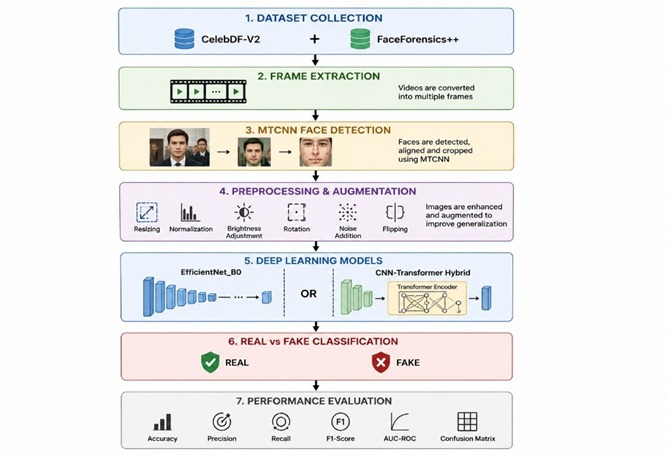
\includegraphics[width=1\textwidth]{3.1.png}
    \caption{Proposed Deepfake Detection Framework}
    \label{fig:dataset_distribution}
\end{figure}


The proposed deepfake detection mechanism is a sequential processing procedure that involves the collection of the datasets, preprocessing, feature extraction, model training, and classification. The proposed system starts by gathering benchmark data such as CelebDF-V2 and Face Forensics++ (FF-C23). Video samples are collected and then converted to image frames by means of frame extraction techniques. Multi-task Cascaded Convolutional Networks (MTCNN) is then used for facial region detection and extraction. Facial images are extracted and subsequently preprocessed and data-augmented (e.g., re sized, normalized, rotated, flipped, and brightened) to enhance the generalization of the model. The deep learning models extract features and classify facial content after pre-processing to differentiate between real and fake content. Lastly, the performance of the proposed framework is evaluated with multiple measures like accuracy, precision, recall, F1-score, ROC-AUC score and confusion matrix analysis. The proposed deepfake classification framework combines the EfficientNet\_B0 and Hybrid CNN-Transformer architectures.

\begin{figure}[H]
    \centering
    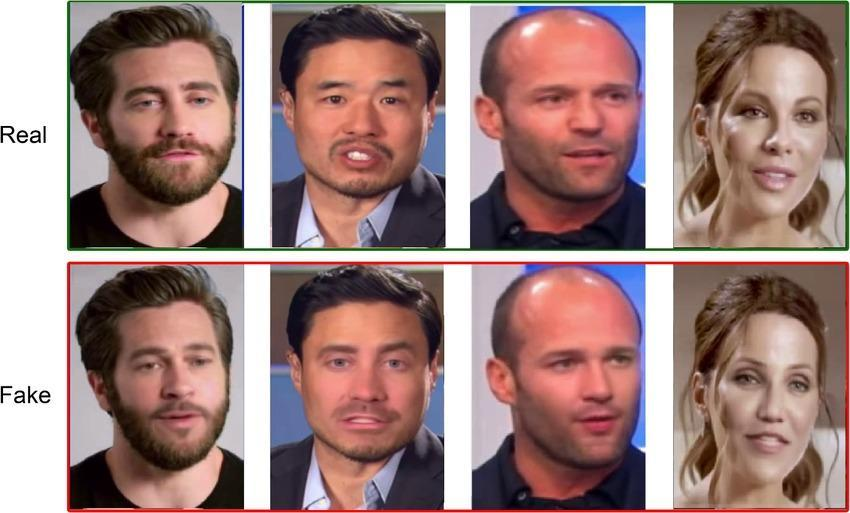
\includegraphics[width=0.8\textwidth]{3.2.png}
    \caption{Comparison of real and deepfake face samples from the CelebDF-V2 dataset.}
    \label{fig:dataset_distribution}
\end{figure}


\begin{figure}[H]
    \centering
    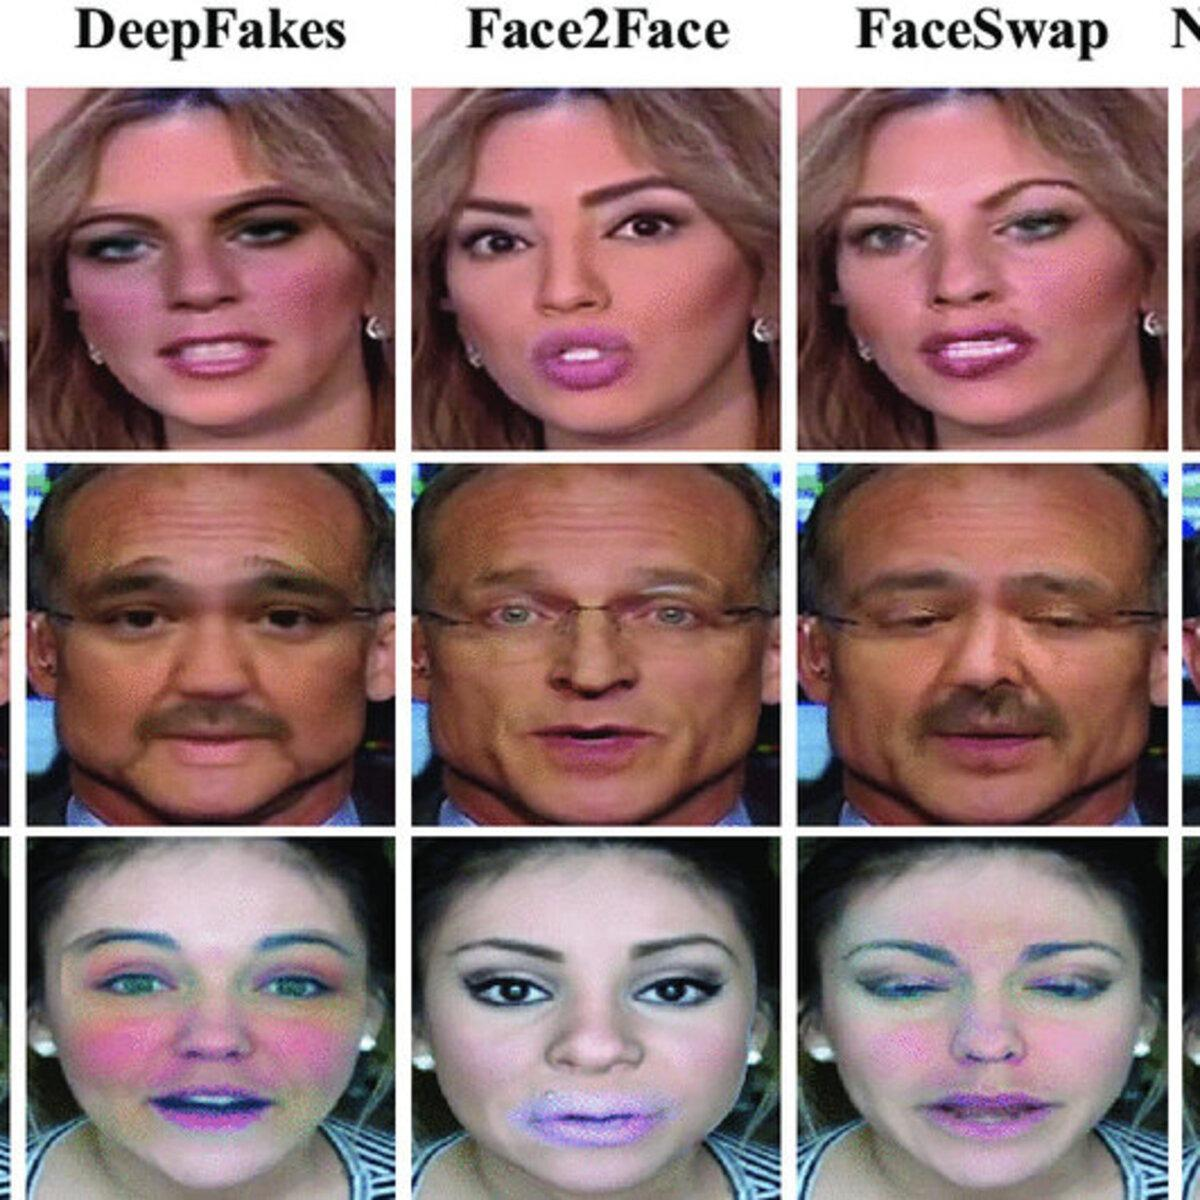
\includegraphics[width=0.8\textwidth]{3.3.png}
    \caption{ Face Forensics++ real vs fake samples}
    \label{fig:dataset_distribution}
\end{figure}

\section{Methodology / Algorithm / Model Description}
The proposed methodology starts with downloading deepfakes datasets from the CelebDF V2 and FaceForensics++ datasets repositories. The frame extraction techniques are used to transform the video into image frames. Image frames are obtained from a video by using frame extraction technique. Multi-task Cascaded Convolutional Networks (MTCNN) is employed for facial region detection and extraction on the extracted frames. The facial images are resized and normalized before being provided as input to the deep learning models.

\begin{figure}[H]
    \centering
    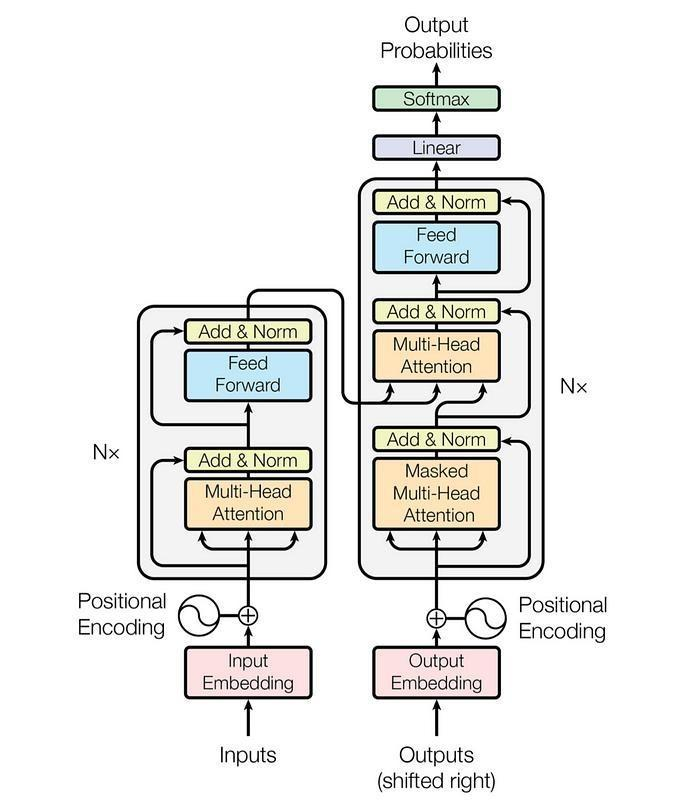
\includegraphics[width=0.8\textwidth]{3.4.png}
    \caption{Transformer model Architecture}
    \label{fig:dataset_distribution}
\end{figure}
\subsection{Preprocessing Pipeline}
The preprocessing stage plays an important role in improving the robustness and generalization capability of the proposed deepfake detection framework. Initially, video samples collected from CelebDF-V2 and FaceForensics++ datasets are converted into image frames using frame extraction techniques. Multiple frames are extracted from each video at fixed intervals to ensure proper facial representation. After frame extraction, Multi-task Cascaded Convolutional Networks (MTCNN) are used for detecting and cropping facial regions from the extracted frames. Face detection helps re move unnecessary background information and allows the model to focus specifically on manipulated facial features. The extracted facial images are resized to a fixed input dimension suitable for the deep learning architectures. Pixel normalization is then performed to scale image intensity values into a standardized range, improving model convergence during training. Several data augmentation techniques are also applied to improve model generalization and reduce overfitting. These include horizontal flipping, random rotation, brightness adjustment, noise addition, and random cropping. Augmentation helps the proposed framework remain robust against variations in illumination, pose, compression artifacts, and image quality degradation. Finally, the processed images are organized into training, validation, and testing sets before being provided as input to the EfficientNet\_B0 and Hybrid CNN-Transformer models for 10 deepfake classification. Data augmentation methods like horizontal flipping, brightness normalization, random crop ping, and adding noise are used to enhance model generalization and prevent overfitting.

\subsection{Working Principle of MTCNN}

MTCNN (Multi-task Cascaded Convolutional Networks) is a deep learning-based face detection and alignment framework used for extracting facial regions from input image frames. It performs face detection through a cascaded architecture consisting of three neural networks: Proposal Network (P-Net), Refinement Network (R-Net), and Output Network (O-Net). The first stage, known as the Proposal Network (P-Net), scans the input image at multiple scales to identify candidate facial regions. It generates bounding box coordinates and facial confidence scores for possible face locations. The second stage, called the Refinement Network (R-Net), further refines the candidate regions obtained from P-Net. It removes false positive detections and improves the accuracy of facial bounding boxes. The final stage, known as the Output Network (O-Net), performs precise facial landmark localization including eyes, nose, and mouth coordinates. It produces the final refined facial region for preprocessing and deepfake classification. The cascaded architecture of MTCNN improves face detection accuracy while maintaining computational efficiency. MTCNN also provides robust facial alignment under different illumination conditions, facial poses, and image quality variations, making it highly suitable for deepfake detection systems. This proposed framework uses two deep learning architectures in deep fake classification. EfficientNet\_B0 is a light CNN architecture that trades off network depth, width and resolution of images. The model has the following advantages: Low computational complexity, fast convergence and efficient extraction of spatial manipulation features from facial images. The second one is a Hybrid CNN-Transformer model architecture, which integrates CNN layers with transformer-based attention mechanisms. CNN layers are used to identify low level spatial characteristics of facial regions, while transformer encoder layers are to capture long-range contextual dependencies and inconsistencies found in deepfake media. Both models are trained by binary classification to classify real and fake facial content. They are then analyzed and compared against each other regarding their effectiveness, computational efficiency and the ability to detect deepfakes.
\subsection{EfficientNet\_B0 Architecture}
EfficientNet\_B0 is a lightweight Convolutional Neural Network (CNN) architecture designed using a compound scaling method that uniformly scales network depth, width, and input image resolution. The model achieves high classification accuracy with significantly fewer trainable parameters compared to traditional CNN architectures such as VGGNet and ResNet. EfficientNet\_B0 is primarily built using Mobile Inverted Bottleneck Convolution (MB Conv) blocks integrated with squeeze-and-excitation optimization modules. The MBConv blocks help reduce computational complexity while preserving important spatial feature in formation from facial images. The architecture starts with an initial convolution layer followed by multiple MBConv stages for hierarchical feature extraction. Global average pooling and fully connected layers are finally used for binary classification of real and fake facial images. One of the major advantages of EfficientNet\_B0 is its lightweight architecture containing approximately 5.3 million trainable parameters. The reduced parameter counts lowers memory consumption, computational cost, and training time while maintaining high classification performance. Therefore, EfficientNet\_B0 is highly suitable for efficient and real-time deepfake detection applications.

\begin{figure}[H]
    \centering
    \includegraphics[width=0.8\textwidth]{3.5.png}
    \caption{Architecture of EfficientNet_B0 12}
    \label{fig:dataset_distribution}
\end{figure}

\subsection{Hybrid CNN-Transformer Architecture}
The Hybrid CNN-Transformer architecture combines the spatial feature extraction capability of Convolutional Neural Networks (CNNs) with the contextual learning ability of transformer models. The hybrid framework is designed to improve deepfake detection performance by capturing both local facial inconsistencies and long-range feature dependencies. In the proposed architecture, CNN layers are initially used for extracting low-level spatial features such as facial textures, edges, blending artifacts, and manipulation inconsistencies from facial images. These extracted feature maps are then converted into sequential feature embeddings and provided as input to transformer encoder layers. The transformer encoder utilizes self-attention mechanisms to analyze relationships between different facial regions and identify global contextual inconsistencies commonly present in deepfake media. Self-attention enables the model to focus on important manipulated regions while learning long-range dependencies across the image. The integration of CNN feature extraction with transformer-based contextual analysis improves the robustness and generalization capability of the proposed framework. The hybrid architecture is particularly effective in detecting high-quality GAN-generated deepfakes where local manipulation artifacts may be less visible.


\begin{figure}[H]
    \centering
    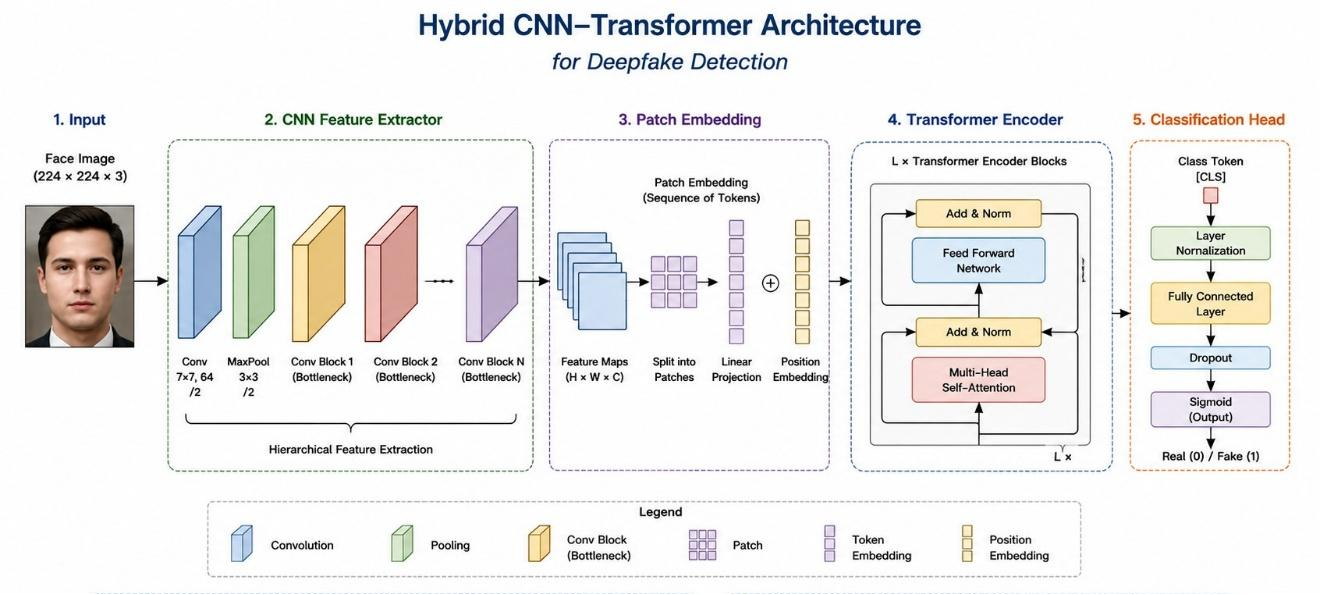
\includegraphics[width=1\textwidth]{3.6.png}
    \caption{Architecture of Hybrid CNN-Transformer Model}
    \label{fig:dataset_distribution}
\end{figure}
\section{Tools, Technologies and Frameworks Used}

The proposed framework was implemented using Python-based deep learning libraries along with GPU acceleration support for efficient model training and evaluation. The tools and technologies used in this research are listed below:

\begin{table}[H]
\centering
\begin{tabular}{|l|l|}
\hline
\textbf{Tool / Framework} & \textbf{Purpose} \\
\hline
Python 3.12 & Programming Language \\
TensorFlow / PyTorch & Deep Learning Framework \\
OpenCV & Image and Video Processing \\
MTCNN & Face Detection and Extraction \\
NumPy & Numerical Computation \\
Matplotlib & Visualization and Graph Plotting \\
Kaggle Notebook & GPU-based Training Environment \\
NVIDIA Tesla T4 & GPU Acceleration \\
\hline
\end{tabular}
\caption{Tools and Technologies Used}
\end{table}


Python was used as the primary programming language for implementing the proposed deepfake detection framework due to its simplicity, flexibility, and extensive support for ma chine learning and computer vision libraries. TensorFlow and PyTorch deep learning frameworks were utilized for designing, training, and evaluating the EfficientNet\_B0 and Hybrid CNN-Transformer models. These frameworks provide GPU acceleration support, pretrained model architectures, automatic differentiation, and efficient tensor computation for large-scale deep learning applications. OpenCV was used for image and video preprocessing operations including frame extraction, image resizing, normalization, facial region manipulation, and video handling. OpenCV provides optimized computer vision utilities that improve preprocessing efficiency. MTCNN was employed for robust facial region detection and alignment. The cascaded architecture of MTCNN enables accurate face localization even under varying illumination conditions, facial orientations, and image quality degradations. NumPy was used for numerical computation, matrix operations, tensor manipulation, and efficient handling of multidimensional arrays during preprocessing and model training. Matplotlib was utilized for visualization and graphical representation of training accuracy, loss curves, confusion matrices, ROC curves, and comparative performance analysis of the proposed models. The experiments were conducted using Kaggle Notebook with NVIDIA Tesla T4 GPU 14 acceleration support. GPU-based computation significantly reduced model training time and enabled efficient large-scale deep learning experimentation.
\section{Performance Metrics / Evaluation Criteria}
The proposed framework was evaluated using multiple performance metrics to analyze classification effectiveness.

\subsection{Accuracy}

Accuracy measures the overall percentage of correctly classified samples.

\[
\text{Accuracy} = \frac{TP + TN}{TP + TN + FP + FN}
\qquad
\tag{3.1}
\]

Accuracy provides the overall classification effectiveness of the proposed framework by measuring the percentage of correctly classified real and fake samples. Higher accuracy indicates better overall deepfake detection capability.

\subsection{Precision}

Precision measures the proportion of correctly predicted fake samples among all predicted fake samples.

\[
\text{Precision} = \frac{TP}{TP + FP}
\qquad
\tag{3.2}
\]

Precision is important in deepfake detection because it measures how many predicted fake samples are actually fake. High precision reduces false positive classifications and improves the reliability of the proposed framework.

\subsection{Recall}

Recall measures the ability of the model to correctly identify fake samples.

\[
\text{Recall} = \frac{TP}{TP + FN}
\qquad
\tag{3.3}
\]

Recall is one of the most significant evaluation metrics in deepfake detection systems because it measures the capability of the model to correctly identify manipulated media. High recall minimizes false negative cases where fake content may remain undetected.

\subsection{F1-Score}

F1-score provides a balanced evaluation between precision and recall.

\[
\text{F1-Score} = \frac{2 \times \text{Precision} \times \text{Recall}}{\text{Precision} + \text{Recall}}
\qquad
\tag{3.4}
\]

F1-score provides a balanced evaluation between precision and recall. It is particularly useful when the dataset contains class imbalance or when both false positives and false negatives are equally important.

\subsection{Confusion Matrix}

The confusion matrix provides detailed visualization of true positives, true negatives, false positives, and false negatives for deepfake classification performance analysis. Confusion matrix analysis provides detailed insight into true positives, true negatives, false positives, and false negatives.

In conclusion, these evaluation metrics collectively provide a comprehensive, multidimensional framework for assessing the proposed model's classification performance. By evaluating overall accuracy alongside the balanced dynamics of precision, recall, and the F1-score, the system ensures both high reliability and minimal false-negative rates. Ultimately, the integration of a detailed confusion matrix analysis validates the model’s robustness and practical viability in accurately discerning sophisticated digital forgeries.

\chapter{EXPERIMENTATION AND RESULTS / APPLICATION/SYSTEM DESIGN AND OUTPUTS }
The experimental work of the project Deepfake Image and Video Detection using Deep Learning was implemented and then executed inside a Python deep learning notebook environment you know the usual. All is gathered in Project.ipynb and the notebook is somewhat using modular experimental setup i.e. it starts with dataset preparation then it continues with face extraction then data loading, then model building and the model training and validation, metric calculation and graph creation, confusion-matrix visualisation and then the comparative analysis. 
\section{System Specifications / Experimental Setup}
\begin{table}[H]
\centering
\begin{tabular}{|l|l|}
\hline
\textbf{Parameter} & \textbf{Value} \\
\hline
Device & cuda \\
GPU & Tesla T4 \\
Epochs & 20 \\
Batch Size & 64 \\
Workers & 8 \\
AMP Enabled & True \\
\hline
\end{tabular}
\caption{Training Configuration Parameters}
\label{tab:training_config}
\end{table}

The notebook got executed in a Kaggle-style GPU setup, you know, that usual environment where everything is already kind of prepared. In the configuration part, it checks what execution device is around using \texttt{torch.device("cuda" if torch.cuda.is\_available() else "cpu")}. In the run itself, the output shows the GPU that was actually available, a Tesla T4, and the whole training loop was set up to lean on CUDA acceleration whenever possible. GPU support mattered a lot here, because both transfer-learning models and transformer-based architectures end up doing those repeated forward and backward passes over a big stack of image tensors. If there was no GPU acceleration then the time needed to train for 20 epochs over more than sixty-five thousand training images would jump quite a bit, and this is even more noticeable for the hybrid CNN transformer model, which basically adds extra sequence modeling over spatial feature patches.

For actually reproducing the project, you’ll want some decent hardware stuff, like a multi-core CPU, enough RAM so image loading doesn’t stall everything, and also enough room for mini-batch preparation. Ideally, you use an NVIDIA GPU that supports CUDA, because it speeds things up quite a bit, though it’s not the only possible route. In the notebook, batch processing was done with a batch size of 64, so in practice a GPU with moderate memory capacity is the safer choice, rather than something very small.

When you look at the models, EfficientNet\_B0 stays relatively light on GPU usage, kind of low key in that sense. But the CNN-transformer model ends up at medium GPU usage since it mixes a deeper EfficientNet\_B3 backbone with transformer encoder layers, so you get the best of both, and also more work in the background. In the final summary produced by the notebook, EfficientNet\_B0 is labeled as faster along with low GPU usage, while the CNN-transformer is labeled medium for both training speed and GPU usage. This mismatch is kind of expected, because the transformer layers run multi-head attention over a sequence of feature patches. That step adds computational complexity compared to a plain convolutional classifier, even if the input pipeline is basically similar.

The overall software setting was basically Python for deep learning and computer vision stuff. We relied on PyTorch as the central training framework, and TorchVision too, for the image transformations, preprocessing pipelines, that kind of thing. For the pretrained EfficientNet models, timm was the go to tool for loading. OpenCV handled video frame reading plus image resizing. For the dataset part, PIL was used for stronger RGB image loading, in that custom dataset class. For face detection we used facenet-pytorch with MTCNN based detection approach, yknow, the usual. Then scikit-learn showed up for the train validation split, and for metric calculation.  
On top of that, there were extra libraries like NumPy, Pandas, Matplotlib, Seaborn and tqdm, for numerical operations, metadata arranging, graph creation, and progress display, sometimes all at once.
The notebook installed facenet-pytorch via pip , which was basically required for the MTCNN face detector. The dependency is kind of significant because the whole project does not train straight on full images or raw video frames, at least not in the straightforward way people might expect. Instead the preprocessing stage tries to isolate the facial area , since most deepfake artifacts show up around facial edges, eyes, mouth, skin texture and even those expression transitions. Once faces are located and cropped ahead of time, the system cuts down the background clutter and kind of nudges the classifier toward the most meaningful region in the input media, rather than letting it waste capacity on irrelevant context.
\section{Parameter Settings / Configuration Details (if applicable)}
The fixed random seed value of 42 is used in all random processes in Python, NumPy, and PyTorch. The benefit gained through such an approach is increased reproducibility because of limited randomness when splitting datasets, initializing neural networks, or applying augmentations. Deep learning experiments are hard to reproduce because of GPU kernel execution and multithreading in data loading, but random seed setting gives the ability to repeat the process with the same conditions.

The image input size was selected to be 224 x 224 pixels. This is an adequate choice since there are many pretrained convolutional neural networks such as different types of EfficientNets where images of the same size are used during fine-tuning and/or training. In the process of preprocessing, images and frames are resized to 320 x 320, then faces are extracted, and the MTCNN face detector uses the \texttt{image\_size = 224} to return face tensors. In the process of data transformation, the size of both training and validation images will be (224, 224). The choice of this size will make it possible to have tensors of shape (3, 224, 224).

The batch size was selected to be 64. With batch sizes that are too small, there is an increased possibility of having more noise in the gradient. Large batch sizes could result in exceeding GPU memory especially for the CNN transformer model. For these reasons, a batch size of 64 is chosen since automatic mixed precision is utilized in this case.

The value of the number of training epochs was fixed to 20 where \texttt{WARMUP\_EPOCHS = 3}. The notebook comments suggest that the epoch number has been increased from 12 to 20 in order to allow enough convergence for the transformer model after warmup. The rationale behind using warmup is to freeze the CNN architecture in the first few epochs and train the classifier network and the other layers unique to transformers such that the pre-trained convolutional neural network architecture converges at a later stage.

AdamW optimizer was used in this notebook. AdamW is an adaptive optimizer, which separates the weight decay from the gradient computation. That is why it can be used for fine-tuning deep learning models since it provides both stable convergence and regularization. For the EfficientNet\_B0, AdamW is used with \texttt{HEAD\_LR = 1e-4} and \texttt{WEIGHT\_DECAY = 1e-4} for all parameters. In case with CNN-transformer architecture, the optimization algorithm works on different parameter groups: the EfficientNet\_B3 backbone is optimized with \texttt{BACKBONE\_LR = 1e-5}; the transformer parts are optimized with \texttt{TRANSFORMER\_LR = 5e-5}; and the classification head – with \texttt{HEAD\_LR = 1e-4}. The choice of these settings is justified by the need to use smaller gradients for backbone layers of pre-trained models and bigger ones for the layers that have to learn new things.
Learning rate is regulated additionally by CosineAnnealingLR schedule with \texttt{T\_max=epochs} and \texttt{eta\_min=1e-6}. The cosine function smoothly decreases learning rate from initial to final small value. This ensures that the network will have greater steps at the early epochs and smaller steps at the later epochs. Learning rate is printed for each epoch in the notebook, which means that the learning rate scheduling mechanism is working while the model is training. This scheduling strategy proves helpful for deepfakes detection as it enables the network to learn overall class separation and then fine-tune boundaries between fake and real images.

Loss Function is CrossEntropyLoss with class\_weights and label smoothing. class\_weights are calculated based on the distribution of the training labels using Counter(train\_df["label"]) with the weight tensor as [total / counts[0], total / counts[1]]. This ensures that both classes contribute equally to the learning process, avoiding bias towards the slightly larger class. The convention of labeling the images for training the deep learning model in the notebook is assigning value 1 for real images and 0 for fake images. Label smoothing is set to 0.1 in order to prevent overfitting of the model. In deepfake detection tasks, label smoothing can be helpful since the artifacts added to the face may be strong enough for some cases but not for others; therefore, using hard labels may be misleading for the model.

The preprocessing step for input data uses ImageNet normalization, with mean \texttt{[0.485, 0.456, 0.406]} and standard deviation \texttt{[0.229, 0.224, 0.225]}. The normalization is applied because the two feature extractors (EfficientNet\_B0 and EfficientNet\_B3) are pretrained using ImageNet from \texttt{timm}. Thus, normalizing the inputs using ImageNet normalization makes sure that the input data is similar to what the pretrained model expects.

Training augmentation consists of resizing, random horizontal flips, random rotations by 15\degree, color jitter with parameters for brightness, contrast, saturation, and hue adjustments, and RandAugment using \texttt{num\_ops = 2} and \texttt{magnitude = 9}. Augmentation helps the model to be exposed to changes in posture, lighting, color balance, and image quality. Augmentation becomes particularly critical when detecting deepfakes since the input image can be from different cameras with various compression rates, different lighting conditions, and varying social media pipelines. Validation and test augmentations differ in that there is no augmentation in them, only resizing, tensor conversion, and normalization.

Mixed precision training was performed via USE\_AMP = True. In mixed precision training, some operations are executed at reduced precision but maintain the stability of training by performing gradient scaling. It helps reduce the consumption of GPU memory and increase the speed of training, especially for deep CNNs and transformer architectures. Gradient clipping was also implemented with clip\_grad\_norm\ using max norm 2.0. It ensures that the training process remains stable by preventing large gradients, especially during the training of transformers.

\section{Implementation Details / Module Description}
\subsection{Dataset Collection Module}

The collection of datasets module works based on the set of configurations for Kaggle input paths: the CelebDF-V2 image dataset can be found at kaggle/input/datasets/pranabr0y/celebdf-v2image-dataset/Celeb\_V2, whereas the FaceForensics++ C23 dataset is available in /kaggle/input/datasets/xdxd003/ff-c23/FaceForensics++\_C23. The CelebDF-V2 dataset contains folders labeled "Train," "Val" and "Test." Both real and fake classes are included within all three folders. In turn, FaceForensics++ is sorted according to the manipulation method. Real videos are recognized as original, while the six folders include various manipulations: Deepfakes, Face2Face, FaceSwap, NeuralTextures, FaceShifter and DeepFakeDetection.

The importance of the module under discussion is that the models must be trained on real and manipulated samples. Using several manipulation methods allows us to train a model for recognition without a bias toward a particular forgery method. Another significance of using the FaceForensics++ dataset is the extension of the project from working with still images to video processing.

\subsection{Data Preprocessing Module}

The preprocessing step takes the raw dataset file and prepares a unified face-image dataset. For CelebDF-V2, the function \texttt{process\_celeb\_images()} iterates across the three splits and two classes. It reads images having extensions like \texttt{.jpg}, \texttt{.png}, and \texttt{.jpeg}; skips every alternate image if \texttt{i \% 2 != 0: continue}; resizes the selected image to 320x320 pixels; uses MTCNN to detect face region; and stores the extracted face in the output directory. Skipping alternate images helps to reduce the computational cost but still maintains a large number of samples.

In case of FaceForensics++, the functions get\_ff\_videos() and process\_ff\_videos() take mp4 files from real and fake video directories. The process\_ff\_videos() function loads the video using OpenCV's VideoCapture object and reads video frames sequentially. It then keeps one frame out of every ten frames if frame\_id \% 10 != 0: continue. Each selected frame is resized to 320x320 pixels, passed through the face extraction function using MTCNN, and stored as a JPEG image. The loop stores at most 10 faces from each video. The Jupyter notebook preprocessed first 200 real and fake videos for training, next 50 real and fake videos for validation, and last 50 real and fake videos for testing.

\begin{figure}[H]
    \centering
    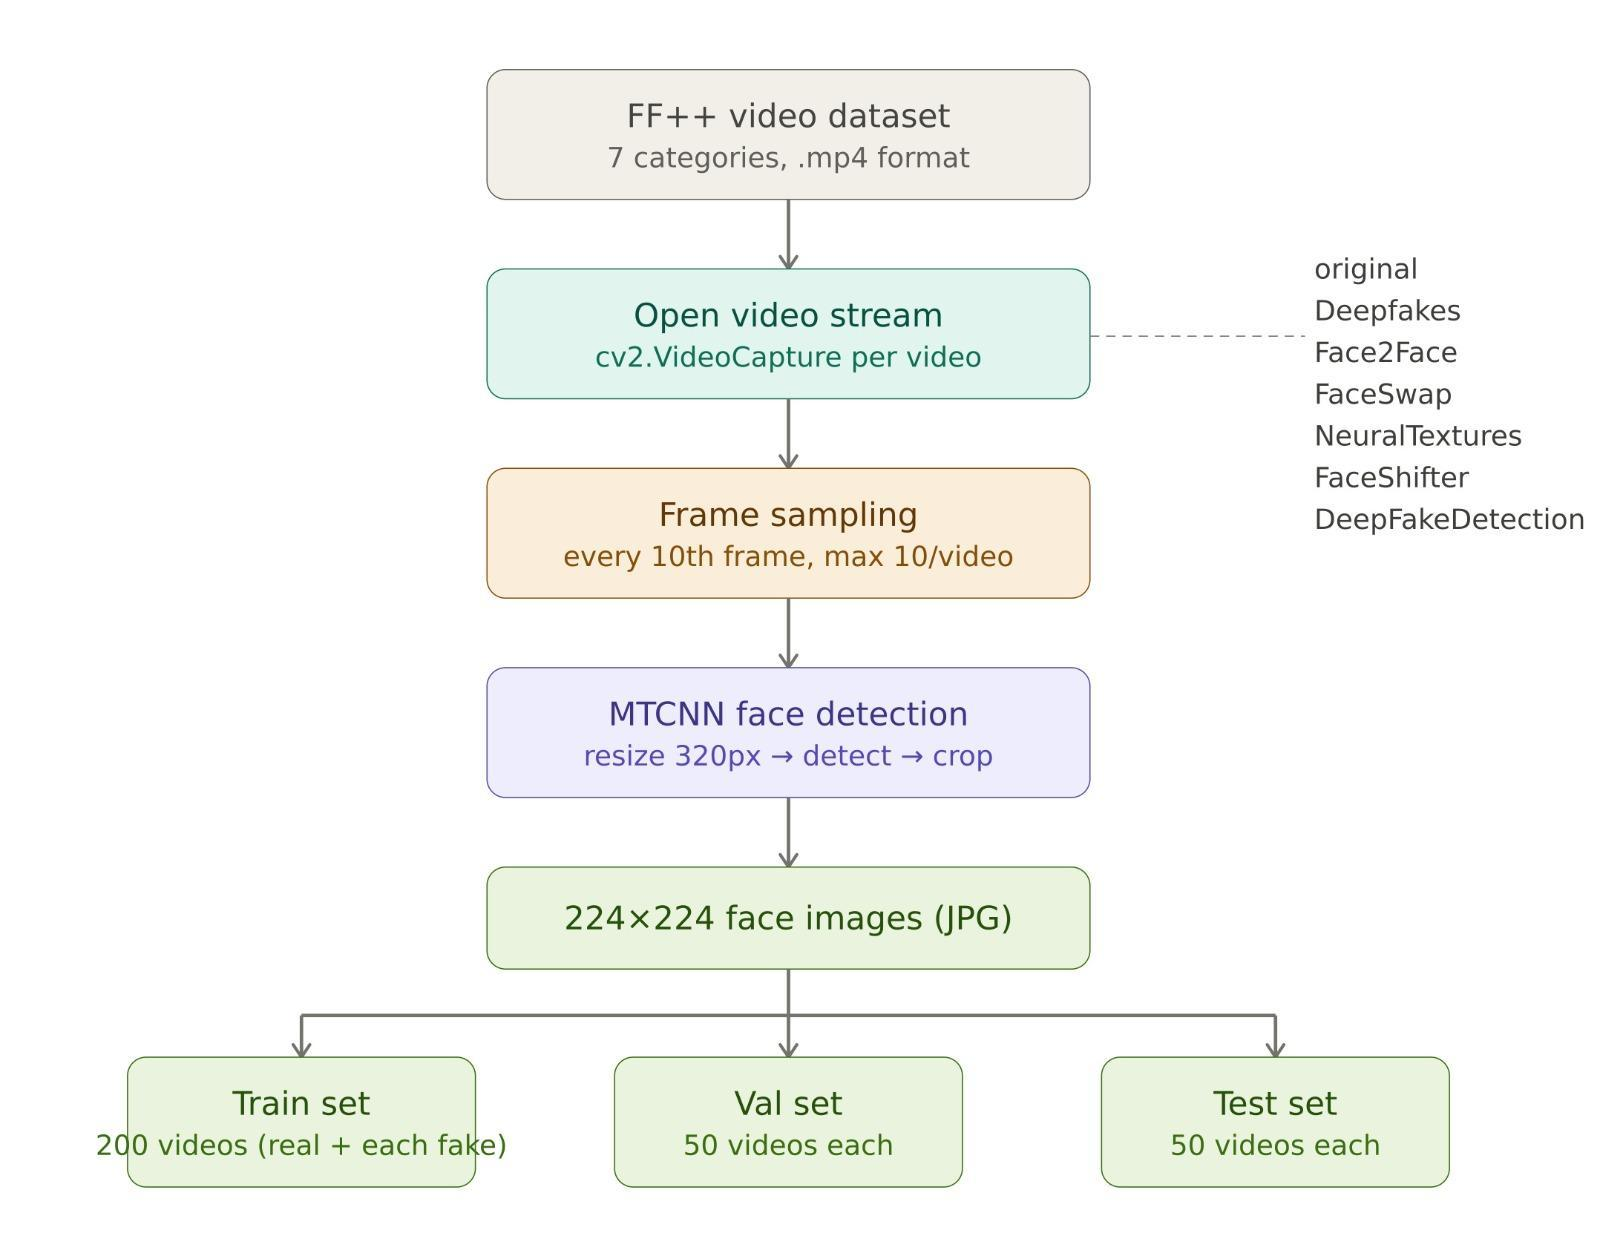
\includegraphics[width=0.8\textwidth]{4.1.png}
    \caption{Video frame extraction workflow from FaceForensics++ videos}
    \label{fig:dataset_distribution}
\end{figure}

The merge\_datasets() function merges both datasets after processing them into the folder /kaggle/working/combined\_data. The structure of the train, validation, and test split along with the classification between real and fake classes will be preserved. Duplicate files found during the merging process will be prefixed with \texttt{"dup\_"} before being saved to avoid accidental overwriting. This step is crucial since the training module requires a single folder containing all data for further processing.

\subsection{Face Detection Module}

The MTCNN algorithm is used to detect faces in the face detection module, using \texttt{facenet-pytorch}. The detector object is created with the following parameters: \texttt{image\_size = 224}, \texttt{margin = 20}, \texttt{keep\_all = False}, and the detected computing device. The margin parameter allows a small part of the surrounding context of the detected face to remain, which can contain valuable information about the boundaries, including artifacts related to blending. The \texttt{keep\_all = False} parameter means that only one face is detected in the image.

The \texttt{extract\_face(img)} function changes the BGR image obtained from OpenCV to RGB, calls the MTCNN method, determines if a face was detected, changes the returned tensor to an image in NumPy, normalizes it, and returns the resulting face image. In case of a failure in the detection process or an exception, \texttt{None} is returned, and the corresponding sample is skipped. This approach does not allow corrupted samples or non-detected faces to be included in the training dataset.

Relevance of this module is extremely significant since deepfake effects manifest themselves mainly within the facial region. In case full image input is provided for the training process, the model may potentially detect spurious information such as background patterns, compression artifacts from the dataset used, or other irrelevant features. This problem is solved through extraction of faces from images.

\subsection{Image Resizing and Normalization}

The image resizing and normalization procedure is achieved via the TorchVision transform methods. Training images are resized to 224 x 224, augmented, converted into tensors, and then normalized based on the ImageNet mean and standard deviation values. Testing images undergo only resizing and normalization steps without any random modifications. Thus, the designed structure ensures that the training process will gain the advantage of diverse images while testing will reflect the behavior of the consistent model.

Normalization plays an essential role since CNNs are pretrained based on ImageNet statistics. Each layer in the EfficientNet learns filter sets based on normalized images. By applying unnormalized faces as input data, we might worsen the transfer learning procedure and slow down convergence. Normalization, therefore, works as a transition between the initial data distribution used for pretraining and the target distribution of faces.

\subsection{CNN Architecture Module: EfficientNet\_B0}

The first model is realized by the class EfficientNetModel, where timm.create\_model("efficientnet\_b0", pretrained=True, num\_classes=0) serves as its backbone. Specifying num\_classes = 0 ensures that the original classification head is discarded, enabling the network to produce feature embeddings. In particular, the EfficientNet\_B0 backbone generates a feature embedding vector with dimension 1280. This feature embedding vector is then fed to a customized classifier model that consists of a linear layer of 1280 → 512, followed by ReLU, dropout (with p=0.4), and a linear layer of 512 → 2.

EfficientNet is an ideal network architecture to be used for this project since it uses compound scaling for a better balance of depth, width, and resolution. The EfficientNet\_B0 is less complex as compared to other CNNs and hence efficient to be trained and utilized for inference purposes. For this particular project, it serves as a great transfer learning algorithm where the convolutional layers detect low-level features such as edges and texture while the classifier differentiates between real and fake faces. Dropout is included to avoid overfitting of the model.

\subsection{EfficientNet-Based Transfer Learning Module}

The use of transfer learning is key to the implementation. In particular, rather than starting with training CNN from scratch, efficient nets with pretrained weights using \texttt{timm} library is used. It is justified in practice since despite the fact that deepfake dataset is large enough, it might not be larger than the dataset necessary for building robust visual features from scratch. Pretraining gives generic vision features, which are then fine-tuned specifically for detecting deepfake images.

The process starts with freezing all backbone parameters for the first three warmup epochs. Then, at epoch 3, the notebook slowly unfreezes the last two blocks from the backbone, while in later epochs, the whole backbone gets un-frozen. That way, the catastrophic effect on pretrained models is avoided, as well as the destabilization of newly created classifier layers before adaptation. One can clearly see it from EfficientNet\_B0 training graph, where the sharp spike in validation accuracy occurs after early warmup epochs and peaks quite early.

\subsection{Transformer / CNN-Transformer Module}

The second model is designed as a class HybridCNNTransformer. This design uses the following line to extract features using timm.create\_model("efficientnet\_b3", pretrained=True, num\_classes=0). In contrast to the classification model based on EfficientNet\_B0, the hybrid model does not apply just a final global CNN embedding to extract features. Rather, backbone.forward\_features(x) extracts a spatial feature map having dimensions (B, C, H, W). Here for the EfficientNet\_B3 model, the number of channels C = 1536. Spatial dimensions are flattened into patches to produce a tensor of dimensions (B, H*W, C).

Then, a LayerNorm function is applied to these vectors to normalize the values. Furthermore, a linear projection function is applied to project vectors into the embedding dimension space with a dimension of 256. A dynamic sequence length is determined using a dummy function. The sequence length, which can be found in the output of the notebook for the designated image size, equals 49. Thus, in this case, the number of patches equals 49, i.e., 7 * 7. A learned positional embedding of dimensions (1, seq\_len, embed\_dim) is used for transformer input.

Transformer encoder contains 2 layers, 4 attention heads, embedding dim = 256, feed forward dim = 512, dropout = 0.3, batch first = True, and norm first = True. Norm first means that the current implementation uses the pre-layernorm transformer, which is considered more stable in training. After the input goes through the transformer encoder to obtain contextualized patch information, global average pooling will be applied to the sequence. Then, this pooled output is fed into a classification head that comprises LayerNorm, Linear (256, 256), GELU, Dropout (0.3), Linear (256, 128), GELU, Dropout (0.2), and Linear (128, 2).

This design intends to leverage both convolution and attention mechanisms. The EfficientNet\_B3 backbone aims to extract hierarchical visual features from the input face image, whereas the transformer encoder aims to learn relationships between regions in the face. Since forgery cues might not be in a single region in the image but are shown as inconsistencies among regions in the face, such as eyes, mouths, skin textures, face borders, and face illumination distribution. The transformer encoder can discover the relationships between these regions after the CNN maps the image to its feature space.

\subsection{Training and Validation Module}

The training function train\_model() takes a model, a model name, and the number of epochs as input parameters. The function dynamically sets the optimizer depending on the presence or absence of a transformer in the model. The function trains the model using the training dataloader and calculates the loss. It uses AMP gradient scaling for backpropagation, gradient clipping, and optimizer update during training. It computes training accuracy and loss after training.

The function also saves the best model checkpoint after every epoch when the validation accuracy improves. The EfficientNet\_B0 model is stored as EfficientNet\_B0\_best.pth, and the hybrid model is stored as CNN\_Transformer\_best.pth. The decision to save the best checkpoint in each case is a crucial aspect of the experiments' design since the chosen model should be selected based on its validation accuracy. The EfficientNet\_B0 experiment obtains its maximum validation accuracy at the end of training. However, the CNN-transformer model continues to improve its performance up to epoch 20.


\subsection{Prediction and Evaluation Module}

The evaluation module makes use of scikit-learn metrics to calculate the accuracy, precision, recall, and F1-score. The evaluate\_model(labels, preds, model\_name) method computes these measures and prints out the classification report. In addition, it creates a confusion matrix and stores it in the graphs folder. As the problem is one of binary classification, the confusion matrix becomes highly insightful because it tells us how many fake images have been wrongly classified as real and vice versa.

As the notebook contains fake examples with labels 0 and real examples with labels 1, the top left entry of the confusion matrix represents the number of fake images that have been accurately identified as fake. Similarly, the top right entry of the confusion matrix represents fake images that have been falsely labeled as real.

\subsection{Video Frame Extraction Module}

Video frame extraction takes the input video files from FaceForensics++ and extracts face images. First, the video file is loaded through the use of OpenCV. The tenth frame of every video file is then selected for further processes. For every video file, a maximum of ten frames will be used. Through this, the chances of data being redundant become low since consecutive video frames are similar.

Even though the output models of the project will end up being image classifiers, the video frame extraction module allows for the detection of deepfakes from video files. This is done by first dividing the video file into individual frames. Then face extraction is done followed by classification.

\subsection{Frame-Wise Classification Module}

Frame-wise classification entails applying the trained real-fake classifier on the extracted video frames. In the implementation of the procedure, the extracted video frames are saved in the same real-fake folder format as images and hence are used for both training and validation. In the deployment scenario, the same idea could be applied to a new video where samples of frames would be taken, detection of the face within these frames would be performed, the trained classifier applied, and the probability of belonging to either class recorded for each frame.

The importance of frame-wise classification is that videos are not equally manipulated across their frames. Some frames could have very high levels of artifacts caused by facial movement, blink, head movement, or occlusion, whereas others could look realistic. Frame-wise classification would enable the system to look at various data points.


\subsection{Final Decision Aggregation Module}

The algorithm does not involve a particular mechanism for making final video-level votes, although such aggregation is possible. The final decision regarding the video can be made via majority vote or based on the average probability of being manipulated. For instance, when most frames are considered to be manipulated, then the video will be marked as manipulated. On the other hand, the average probability of being manipulated can also be checked against some pre-defined threshold level; if higher, then the video is considered manipulated.

Such aggregation is important as it aggregates frame-level decisions into video-level one and provides increased robustness of the classifier due to the possibility to ignore a handful of incorrectly classified frames when making a final decision. In practical implementations, however, probability averaging is usually preferable since it retains more information than simply classifying the video as manipulated.

\begin{figure}[H]
    \centering
    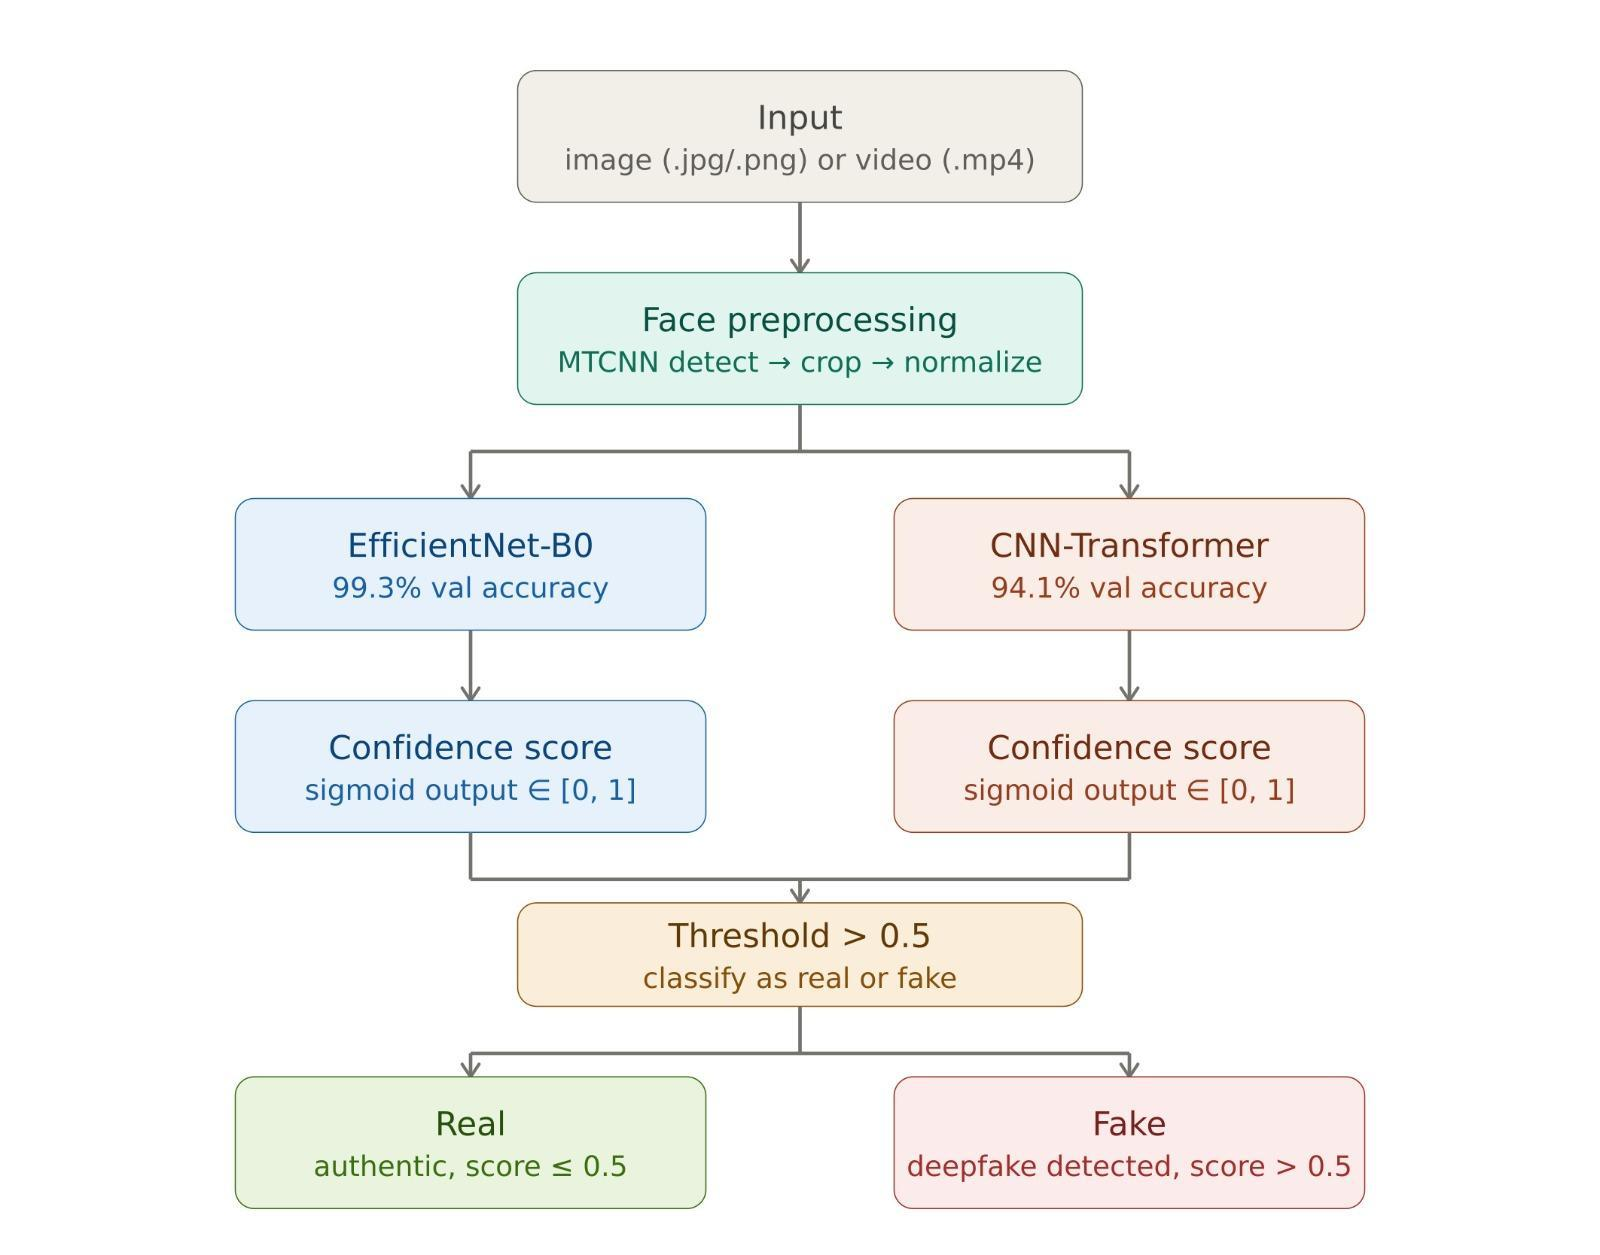
\includegraphics[width=0.8\textwidth]{4.2.png}
    \caption{End-to-end system flowchart from input image/video to final real/fake decision}
    \label{fig:dataset_distribution}
\end{figure}


\section{Results and Outputs}

Training curves, validation curves, confusion matrices and a final metric comparison chart have been obtained from the experiment conducted. Some of the files that have been generated from the experiment include accuracy and loss charts for EfficientNet\_B0 model, accuracy and loss charts for the CNN-transformer model, individual confusion matrices, one confusion matrix chart and a final metric comparison chart.

\subsection{EfficientNet\_B0 Accuracy Result}

The EfficientNet\_B0 model had a maximum validation accuracy score of 99.32\%. From the training logs, the EfficientNet\_B0 model started off with 65.72\% training accuracy and 67.66\% validation accuracy during epoch 1. However, during the initial warm-up phase, there was an incremental change. It is notable that the most significant jump in performance came when the backbone started fine-tuning, which resulted in a validation accuracy of 88.45\% for epoch 5 and 95.30\% for epoch 6.

\begin{figure}[H]
    \centering
    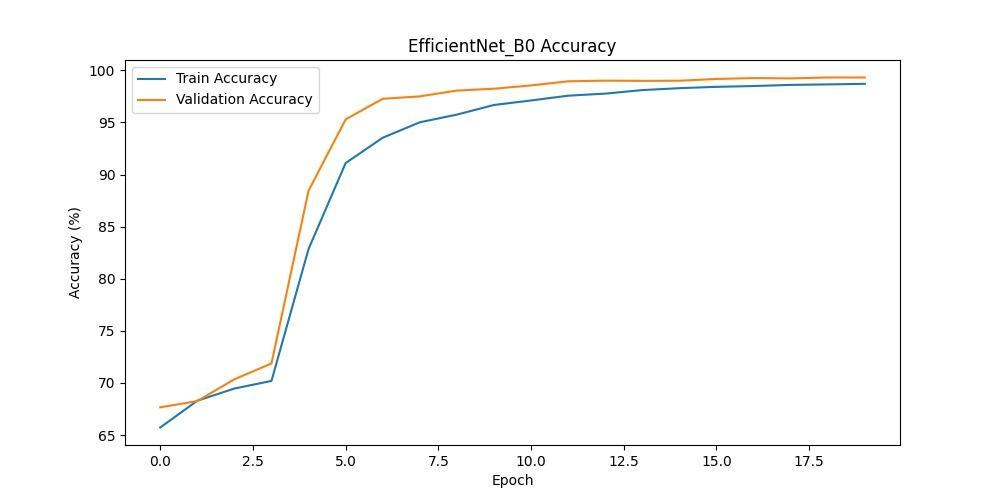
\includegraphics[width=0.8\textwidth]{4.3.png}
    \caption{EfficientNet B0 Accuracy }
    \label{fig:dataset_distribution}
\end{figure}

The graph shows that the transfer learning approach worked very well for the provided data. The difference between the training and validation accuracies became smaller during later epochs, implying that the model did not learn by heart the training dataset but was able to generate meaningful facial features that were applicable to the validation dataset.

\subsection{EfficientNet\_B0 Loss Result}

The EfficientNet\_B0 loss consistently reduced during the training process. In epoch 1, it showed a training loss of 0.6325 and a validation loss of 0.6183. During epoch 6, it was 0.3437 for training and 0.2803 for validation. In epoch 20, the training and validation losses were respectively 0.2231 and 0.2126.

\begin{figure}[H]
    \centering
    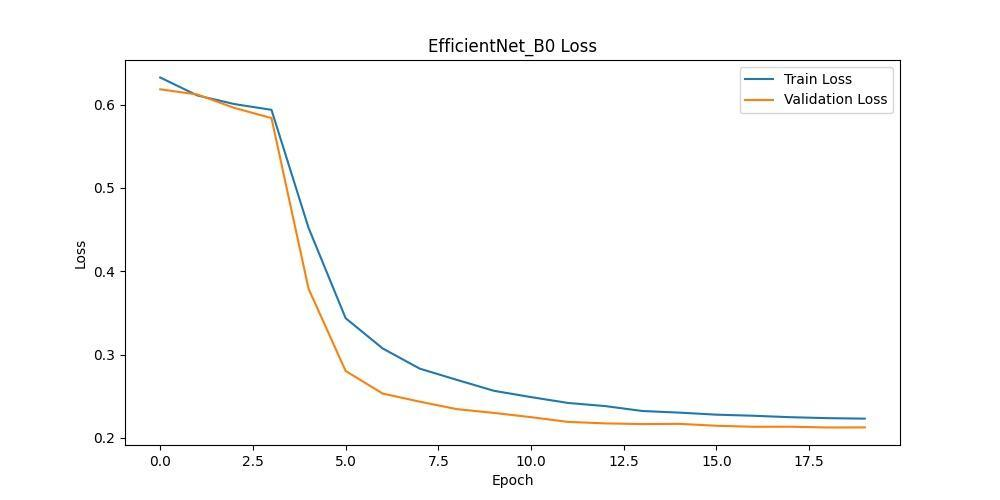
\includegraphics[width=0.8\textwidth]{4.4.png}
    \caption{EfficientNet B0 Loss}
    \label{fig:dataset_distribution}
\end{figure}
From the graph above, the learning trend was showing that the model was separating the classes' boundaries better and better as time went on. It is possible that the validation loss was always either slightly lower than or equal to the training loss at the latter stages due to training with augmentations, dropout, and label smoothing. In other words, since the training data are artificially created and there is regularization, training could have been more difficult.

\subsection{CNN-Transformer Accuracy Result}

CNN transformer was able to attain the highest validation accuracy score of 94.11\%. CNN transformer begins with a training accuracy of 64.41\% and validation accuracy of 67.90\% at epoch 1. The accuracy improved gradually from epoch 1 to epoch 20. It had an accuracy score of 79.87\%, 90.05\%, 93.36\%, and 94.11\%.

\begin{figure}[H]
    \centering
    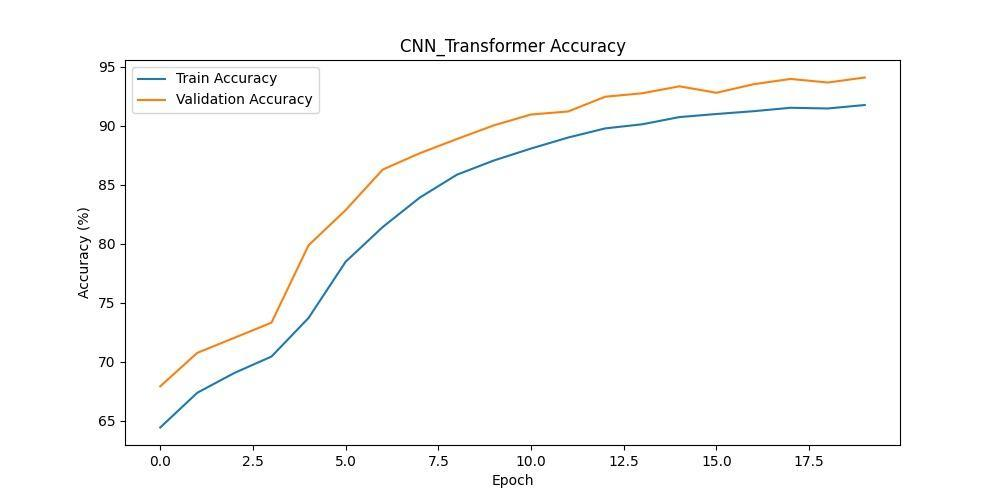
\includegraphics[width=0.8\textwidth]{4.5.png}
    \caption{CNN Transformer Accuracy}
    \label{fig:dataset_distribution}
\end{figure}

There is a more gradual but consistent trend for the learning process as compared to EfficientNet\_B0. This can be anticipated due to the more complex architecture of the hybrid model which consists of an EfficientNet\_B3 base, projection layers, position encodings, transformer encoder layers, and a more complex classifier. Learning through the transformer takes more training time to grasp the spatial relationships among the face region feature vectors.

\subsection{CNN-Transformer Loss Result}

CNN-transformer model started from training loss of 0.6391 and validation loss of 0.6107. Training and validation losses were decreasing during the training process; after 10 epochs, training loss was 0.3956, while validation loss was 0.3538. After 20 epochs, training loss was 0.3260, while validation loss was 0.2933.

\begin{figure}[H]
    \centering
    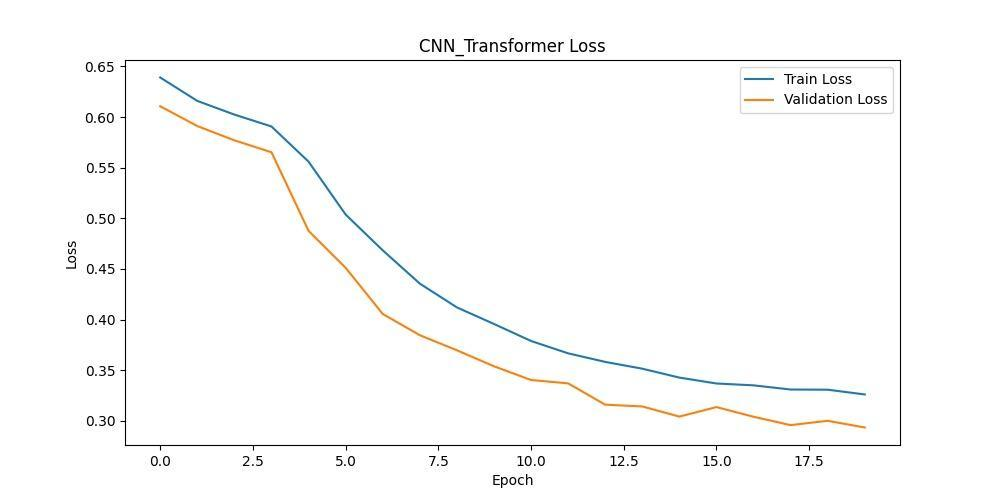
\includegraphics[width=0.8\textwidth]{4.6.png}
    \caption{CNN Transformer Loss}
    \label{fig:dataset_distribution}
\end{figure}

From the graph above showing losses, we can observe that the hybrid model had acquired some features since it took more time to converge as compared to EfficientNet\_B0. Also, validation loss continued being less than the training loss for several epochs, and this is due to effective data augmentation and dropout during training. Since the accuracy of this model was relatively low when compared to EfficientNet\_B0, we can conclude that the transformer needed more data or better fine-tuning.

\subsection{Confusion Matrix for EfficientNet\_B0}

From the confusion matrix figure, it is observed that the model EfficientNet\_B0 classified 8187 out of the total 8251 fake samples as fake, while only 64 out of the total were misclassified as real. Likewise, 8139 out of the total 8187 real samples were classified as real, whereas 48 samples were misclassified as fake.

\begin{figure}[H]
    \centering
    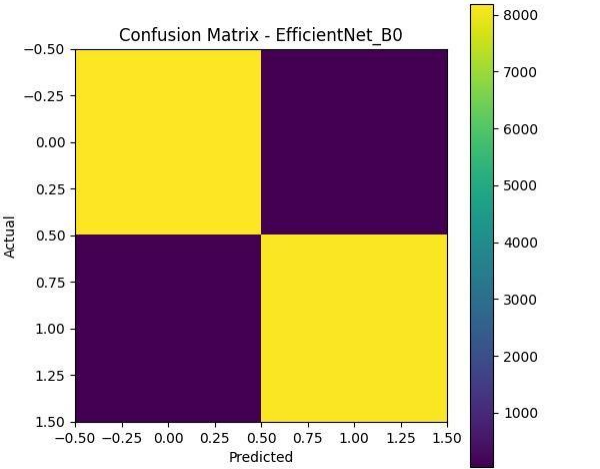
\includegraphics[width=0.8\textwidth]{4.7.png}
    \caption{Confusion Matrix - EfficientNet B0}
    \label{fig:dataset_distribution}
\end{figure}

\begin{figure}[H]
    \centering
    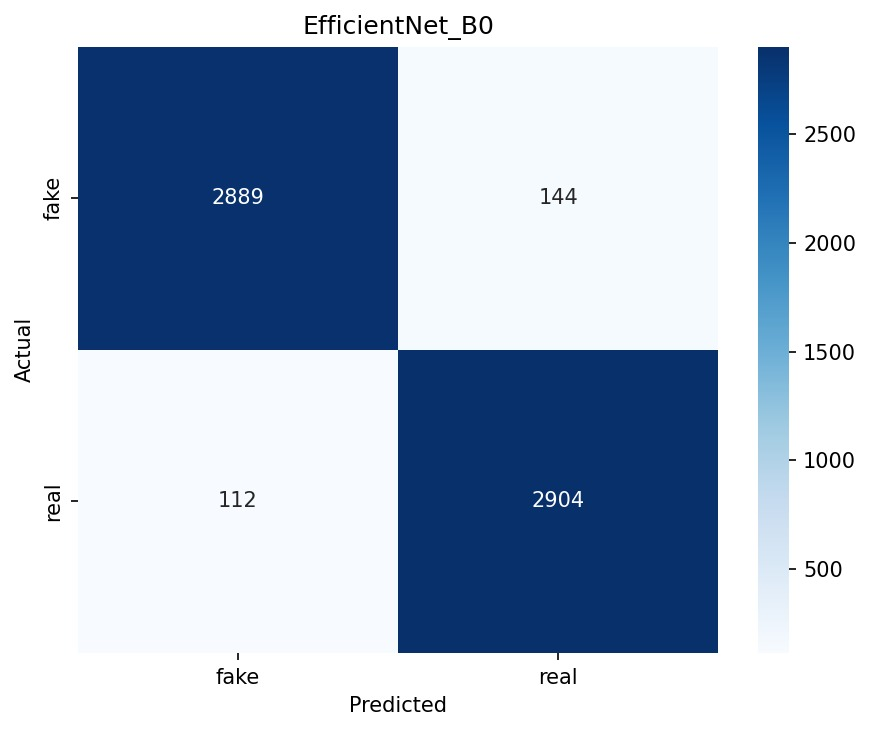
\includegraphics[width=0.8\textwidth]{4.7.1.png}
    \caption{Confusion Matrix - EfficientNet B0(Testing Data)}
    \label{fig:dataset_distribution}
\end{figure}

In the case of deepfake recognition, false positives and false negatives will differ in their effects on the outcome. A fake image incorrectly classified as a real one will be hazardous, while a real image wrongly classified as a fake image may erode confidence in authentic images. According to the EfficientNet\_B0 confusion matrix, there are very few occurrences of such errors in this scenario.

\subsection{Confusion Matrix for CNN-Transformer}

The CNN-transformer confusion matrix has 7584 false samples that are recognized as false and 7885 true samples that are recognized as true. However, it has 667 false samples that are incorrectly categorized as true and 302 true samples that are incorrectly recognized as false.

\begin{figure}[H]
    \centering
    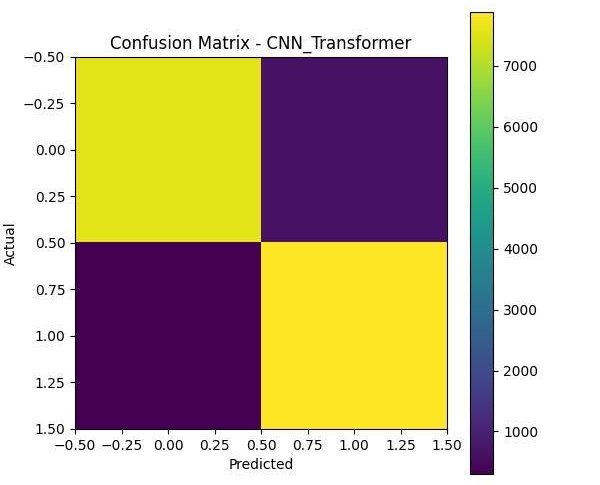
\includegraphics[width=0.8\textwidth]{4.8.png}
    \caption{Confusion Matrix - CNN Transformer}
    \label{fig:dataset_distribution}
\end{figure}

\begin{figure}[H]
    \centering
    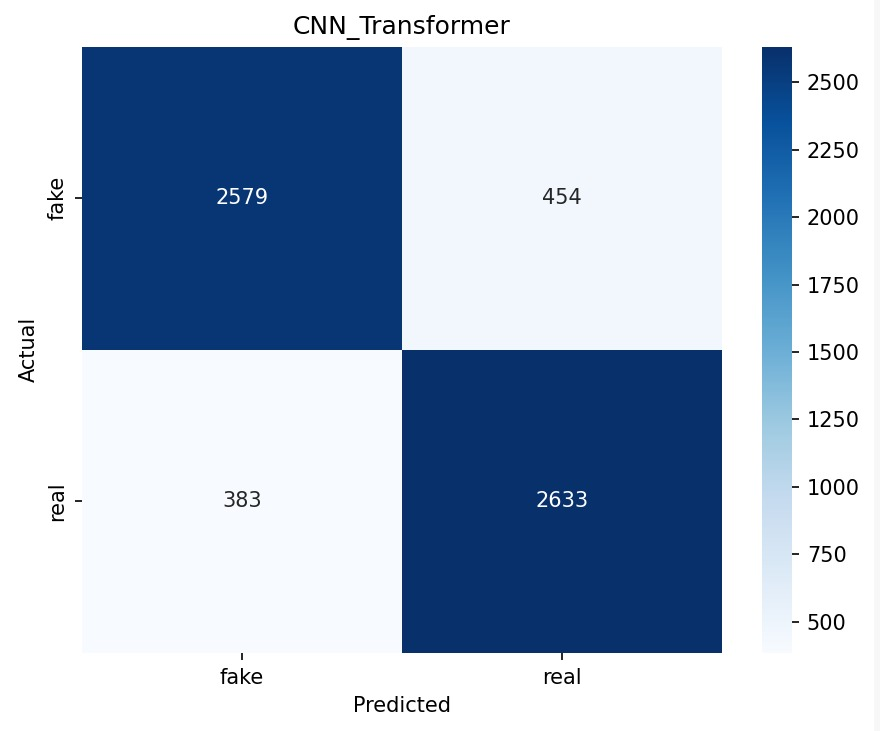
\includegraphics[width=0.8\textwidth]{4.9.1.png}
    \caption{Confusion Matrix - CNN Transformer(Testing Data)}
    \label{fig:dataset_distribution}
\end{figure}

From this confusion matrix, it can be observed that the CNN-transformer model achieves better recall on the true samples than the false samples. It makes more mistakes when categorizing false samples into true samples, compared to the EfficientNet\_B0 model. Thus, even though the transformer-based approach is effective in learning relationships, its decision-making process is relatively less stringent when dealing with false samples.


\subsection{Final Metric Comparison}

This graph presents the comparison of various performance measures between the two models. EfficientNet-B0 obtained close to 99.3\% (Validation Accuracy) and 98.66\% (Training Accuracy) for the key performance measures, whereas the CNN-transformer performed at 94.1\% (validation accuracy) and 91.77\% (training accuracy), 94.2\% precision, 94.1\% recall, and 94.1\% F1 score. The results from the printed output in the notebook indicate EfficientNet-B0 having a performance of accuracy = 0.9932, precision = 0.9922, recall = 0.9941, and F1 score = 0.993


\begin{figure}[H]
    \centering
    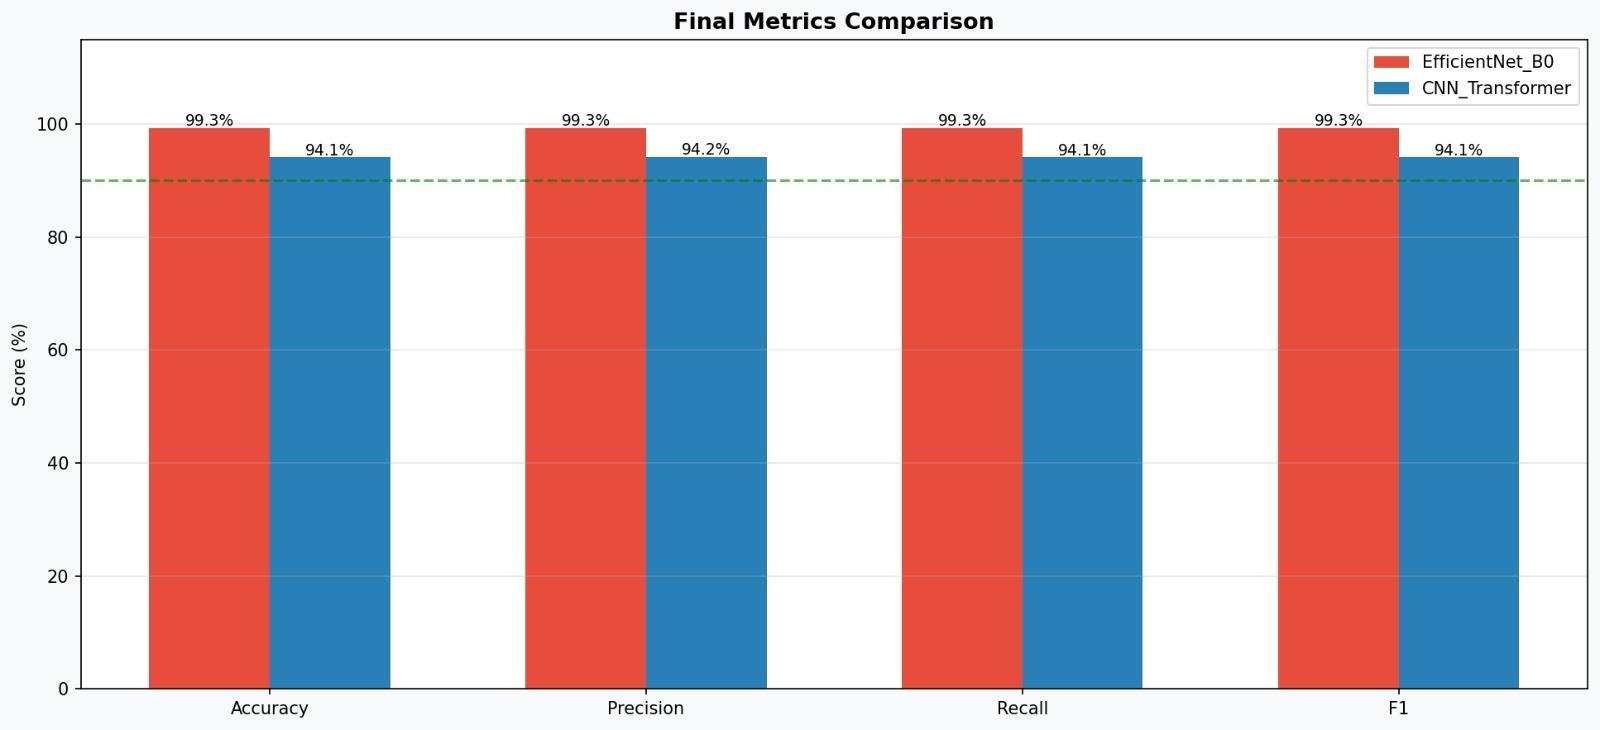
\includegraphics[width=0.8\textwidth]{4.10.png}
    \caption{Final Metrics Comparison}
    \label{fig:dataset_distribution}
\end{figure}

\begin{figure}[H]
    \centering
    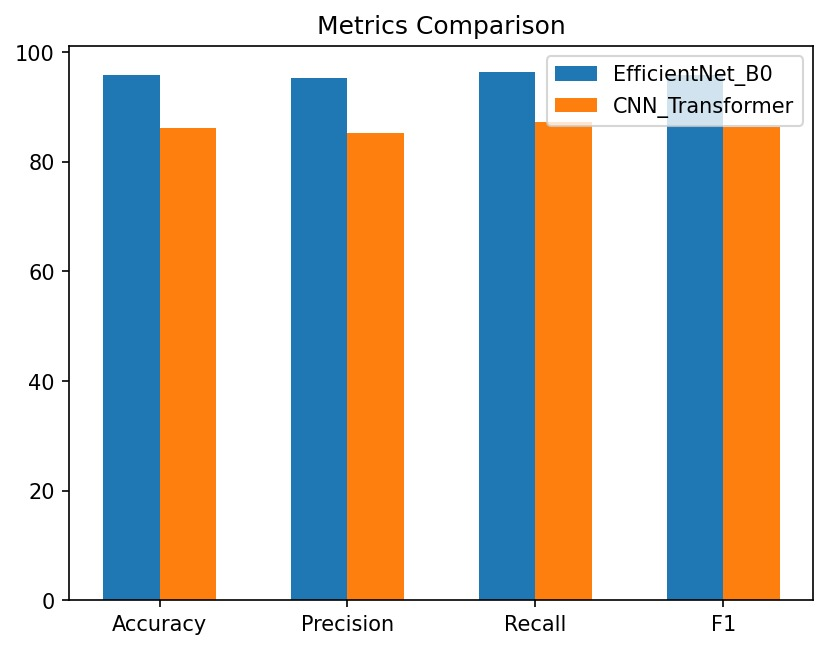
\includegraphics[width=0.8\textwidth]{4.11.png}
    \caption{Final Metrics Comparison for testing data}
    \label{fig:dataset_distribution}
\end{figure}

The result demonstrates that EfficientNet\_B0 is better than the CNN-transformer in this particular application. Nevertheless, the CNN-transformer also demonstrated very good results above 94\%. It is evident that spatial modeling using an attention mechanism was correct, although the poorer result might be attributed to greater model complexity or optimization issues.

\section{Result Analysis and Validation}

From the results obtained from the experiments, it can be seen that the implemented system is capable of detecting deep fake face images accurately. From the available models currently implemented, the best one is the EfficientNet\_B0, with the best validation accuracy being 99.32\%. The high validation accuracy shows the efficiency of transfer learning together with the usage of face image pre-processing, loss weighting and image augmentations. EfficientNet\_B0 model had the highest validation accuracy since it uses an efficient architecture that is suitable for image classifications and local texture cues.

CNN-Transformer got a validation accuracy of 94.11\%. Although it was not able to perform as good as EfficientNet\_B0, it still produced relatively accurate predictions. The design of the CNN-Transformer model was aimed at the learning of the relationships between CNN features. The constant improvements on loss and accuracy show that it was able to learn the features well. The transformer model would be applicable in cases whereby the manipulations are based on the relationship between patches of faces and not just local texture cues.

Confusion matrices provide additional insights beyond accuracy metrics. EfficientNet\_B0 had only 112 total errors among all samples, i.e., 16438 samples, compared to 969 total errors by CNN-transformer. EfficientNet\_B0 had 64 and 48, respectively, errors of assigning fakes to real and vice versa. In contrast, CNN-transformer had 667 errors of assigning fakes to real samples and 302 real-to-fake ones. As per the threat posed by deepfakes, fake-to-real mistakes matter much more since it allows attackers to get their manipulations past detectors. Thus, while CNN-transformer had a high ability to catch real samples, it cannot be considered superior because the main objective is detecting deepfakes.

From the loss and accuracy charts of both models, it is clear that training helped improve their performance. Particularly, EfficientNet\_B0 gained greatly once the backbone was unfrozen, proving that fine-tuning layers pretrained on ImageNet data was needed to produce good results. In comparison, CNN-transformers improved slowly due to the difficulty of learning attention patterns of transformers as opposed to CNN features. No model diverged excessively or behaved erratically, proving that training hyperparameters were adequate.

Generalization seems solid according to validation performance. Using the face extraction tool MTCNN removed irrelevant variability caused by background, while augmentation helped increase robustness to lighting conditions, rotation, coloring, and horizontal flipping. Combining CelebDF-V2 and FaceForensics++ provided robustness due to using two kinds of samples - images and video frames.

Nevertheless, there are certain limitations. First of all, the validation procedure relies on processing already existing face images, which can differ from deepfakes in terms of greater compression, unknown manipulation techniques, poorer resolution, occlusion, multi-face, profile, and other types of variability. Another limitation concerns not building a complete video decision-making model, but evaluating frame classification. Though frame-wise classification makes sense due to the way the decision function was built, there is still space for improvement here, as aggregating functions should be implemented later. Besides, as the MTCNN detector ignores samples without faces, this approach leads to better training quality but lower coverage in some cases.

In summary, the experimentation results show that the proposed solution was able to effectively implement a deep learning pipeline for distinguishing between real and fake faces. The project highlights data pre-processing, face recognition, transfer learning, a CNN-transformer based approach, regularization, metric computation, and visualization of the results. From the experimental observations, the most effective model at the current stage is EfficientNet\_B0, while the alternative model – the CNN-transformer – has technical value and could be further improved with additional training and hyper-parameter tuning.


\chapter{ETHICAL, SOCIAL \& SUSTAINABILITY CONSIDERATIONS}
\section{Ethical Consideration}
The fast development of artificial intelligence technology has helped immensely in generating, altering and synthesizing digital media content. The deep learning techniques like GANs, Diffusion models and Face-Swaps help create realistic manipulations of images and videos which can easily be passed off as genuine pieces by normal people. Even though these techniques have legitimate uses in movies, education, entertainment, making life easier for disabled people and creative media content creation, the misuse of these technologies for impersonating a person, spreading disinformation or altering public opinions is unethical and should be prevented at all costs. The purpose of this project ``Deepfake Image and Video Detection using Deep Learning'' is to find a solution to this ethical dilemma.

Another crucial ethical issue related to deepfakes involves their potential use for spreading misinformation. Media is now one of the most common sources of information for modern people, and photos and videos are regarded as a form of visual proof that an event actually happened. This assumption is undermined with the advent of deepfake technology, which allows creating visually convincing content depicting events that did not happen in reality. The use of such content could be employed to manipulate people into thinking something they should not, shape political views and voting preferences, make false allegations, manipulate the stock market, among other things. With this in mind, it becomes evident that deepfake detection has ethical significance since it ensures the authentication of content.

Another ethical consideration is identity abuse. Deepfakes typically involve the use of one’s facial features, voice, or physical resemblance without their consent. This poses an ethical challenge since people’s personal rights to self-respect and autonomy are violated. An individual is portrayed in an event that did not happen or an action that they did not perform. Such an artificial portrayal might lead to emotional trauma, social humiliation, career damage, or even legal implications. The key ethical concept in this case is that of consent. An individual’s identity should not be included in a media creation without their consent.

Privacy is another important consideration in the development of deepfake detection technology. Because the system operates on facial images and video frames, it handles biometric data. Facial features constitute private data since they provide details that identify personal information such as identity, emotions, age, gender, and other traits. Thus, all deepfake detection systems must take care of the data they handle. The collection of datasets, model training, and system deployment must be done in a manner that respects privacy protocols. This includes the use of legitimate data sets, restricted access to images in storage, minimal collection of private information, and non-exploitation of face samples acquired from the data.

In developing an AI solution responsibly, fairness and bias need to be accounted for properly. An AI model that uses a deepfake detector could possibly yield better predictions on some groups compared to others because of the lack of demographic diversity in the training dataset. In cases where there is greater representation in the data of some ages, ethnics, lighting or quality cameras, the AI model is more likely to yield poor predictions for some groups. This poses a risk of unfairness when it comes to using the AI system, which is unethical in particular applications like media, investigations and platform moderation. Evaluation is key in ensuring fairness, and class-wise testing is also needed.

Ethical considerations are important in both cases. False positive means that real media is erroneously recognized as a deepfake one. It will undermine the credibility of people who share their own videos or pictures – they can be anyone from a regular witness to the famous journalist. False negative implies that altered media is not recognized as a deepfake and, therefore, will spread freely. In deepfake detection, the former two errors are critical. For ethical operation of the algorithm, we should regard its predictions as advisory inputs but not the final decisions. People working on the task should use it as an assistant, but never rely solely on the prediction results.

\section{Social Impact and Societal Relevance}

It is more relevant than ever before for deepfake detection to be socially relevant due to the increasingly crucial roles played by digital media in communications, politics, journalism, education, security and personal interactions. Visual media are now part of people's daily interactions on social networking sites, news portals, messaging apps and even video sharing sites. The validity of these visual media has become an essential part of social trust. A research project involving the detection of deepfake images and videos is relevant to society.

Misinformation is among the gravest social issues associated with deepfakes. Videos can be manipulated to present public figures saying things they never did, attending events they never attended or expressing opinions that could lead to negative consequences. These videos can be disseminated across social networking sites within minutes, before anyone can take action to counter them. When such videos appear in times of political significance, they may contribute to social division and even undermine democratic processes. An effective deepfake detection tool will enable faster detection and reduce misinformation.

Finally, deepfake technology may affect social media authenticity. Applications for video distribution, social networking sites, and instant messaging tools allow for quick dissemination of content posted by users. Although this aspect helps in faster communication, the task of monitoring this process raises many questions. It is impossible to manually verify the legitimacy of each photo or video that users upload onto the platform. However, with the development of automated deepfake detection software, moderators will be able to flag any potentially manipulated material for additional analysis. The proposed system will alleviate the work of human reviewers and contribute to maintaining platform safety during significant events, such as elections, wars, or other emergencies.

Moreover, deepfake detection may have applications for cybersecurity. Deepfakes are useful when it comes to conducting social engineering, identity theft, spoofing activities, and business email compromise attacks. For instance, an attacker may use deepfake videos or voiceovers to pretend to be a CEO or another employee within an organization and make financial requests. Deepfake images may also facilitate social engineering attacks by exploiting vulnerable identity verification protocols. As a result, deepfake detection turns into a cybersecurity technique, which helps identify facial content manipulation.

One of the other application areas is digital forensics. Forensic investigators increasingly face instances of digital evidence, including images and videos. Authenticity is very important in both legal and investigative applications. Deepfake detectors may prove helpful for forensic experts who need a first technical estimate regarding the manipulative nature of the media sample under analysis. Nevertheless, the results provided by the models in the legal domain should be interpreted cautiously. There should always be a specialist who will analyze the model outputs, document the investigation process and ensure its validity.

Deepfakes also impact journalism significantly. The news agencies are responsible for verifying any media content prior to distribution. Publishing a single fake picture or video without verification will damage the reputation of the news agency and lead to misinformed people. Deepfake detectors could aid journalists in the media verification pipeline. They might prove helpful when checking submitted pictures and videos, social media posts or even viral videos. It becomes especially important in cases of breaking news stories, when journalists feel the urge to publish news as soon as possible but lack sufficient time to verify the sources of media content.

Law enforcement organizations could also make use of the deepfake detection technology. Deepfakes can be involved in cyber harassment, blackmailing, defrauding, defamation and identity theft. If individuals suffer as victims of manipulated videos, they might need assistance in order to prove their case. Deepfake detection would be able to assist in the identification of manipulated content, as well as aid in investigation of the criminal activity.

Moreover, deepfake detection helps protect one’s personal reputation and mental health. Individuals victimized through manipulated media can face severe consequences in terms of emotional stress, social exclusion, or even professional life. The problem becomes even more severe in situations when an individual faces deepfake-based cyber-harassment or online bullying. Deepfake detection can aid those affected and show that malicious content was actually manipulated.

Raising public awareness is also a critical societal consequence of projects such as the current one. Such projects raise public awareness regarding the dangers of using synthetic media. Many people often believe that videos serve as irrefutable evidence of reality. The increased accessibility of technology for the creation of deepfakes will make it essential to understand that videos are sometimes used to spread manipulation with the aid of artificial intelligence. Therefore, technical projects aimed at the identification of deepfakes play an important role in raising public awareness regarding deepfakes.

\section{Sustainability Consideration}

The concept of sustainability in relation to this research project can be viewed in terms of three broad categories: computational sustainability, operational sustainability, and sustainability of society in the long run. Deep learning models may demand considerable computational resources when developing and using them for processing data sets that consist of images and videos. On the other hand, automated deep fake detection will contribute to sustainability due to its ability to cut down the cost of social and institutional damages caused by digital fraud and deception.

With regard to the sustainability aspect, the researchers chose to implement transfer learning technology into their work because there is no need to start building a deep convolutional network model from scratch. There is an obvious computational sustainability since the pre-trained model already contains features learned during training. Moreover, fine tuning of EfficientNet models demands less computing power and fewer training epochs than training a completely new model. In particular, the model EfficientNet\_B0 seems to be particularly important since it offers high accuracy along with low GPU usage and faster training. 

The utilization of EfficientNet also demonstrates a sustainable model design process. The architecture of EfficientNet is engineered in such a way that it optimizes its depth, width, and input resolution. It allows obtaining an excellent level of performance without wasting too many parameters. An efficient model is preferred during actual implementation due to the reduced inference cost, lower energy use, and fewer requirements for hardware. A light yet accurate model can be implemented in cloud servers, corporate networks, or even edge devices.

In terms of computational complexity, the CNN-transformer model is not sustainable. However, it might be an appropriate subject for further investigation. Transformers might be capable of detecting spatial relationships that simple CNN classifiers are unable to identify. Nevertheless, it should be assessed whether the increase in performance is worthwhile compared to the increased computational load. At present, EfficientNet\_B0 shows better results than the CNN-transformer and is also faster. Thus, the former model is more sustainable.

The preprocessing methodology used also has an impact on sustainability. The model is trained on specific frames selected from the video rather than training on the entire video stream. For FaceForensics++ data set, the notebook processes every tenth frame and only saves up to ten frames from the video, which includes the detected face. This is necessary to avoid duplicate work, where highly similar frames are analyzed separately from one another. It cuts down the amount of training data, thus saving memory space, storage and time. The use of the face extraction method additionally excludes unnecessary data, such as backgrounds.

The use of automated moderation systems is a factor that affects the sustainability of moderating harmful and altered content on social networks. Manual content moderation cannot be sustained as there is an excessive amount of media uploaded to social networking sites. Moderators often undergo psychological problems when subjected to continuous exposure to manipulated and harmful content. AI content detection would allow for automated prioritization of suspicious content requiring further review.

Long-term digital security is intertwined with sustainability. With the increased accessibility of deepfake techniques, there will be a need for sustained systems that can detect authentic information. A sustainable deepfake detection algorithm must be flexible and updatable to accommodate any changes in data sets and techniques used to manipulate them. The modularity of the current project aids in achieving this since each phase of the process is handled by different parts. This makes it easy to update future versions of each module individually.

Sustainability of data is another consideration. The deepfake detector model needs to train and test using a dataset that represents modern manipulation techniques. Using an old-fashioned deepfake method to train the model will result in poor performance when evaluating new generative techniques. As a result, dataset update, training, and evaluation of models need to be done repeatedly for continuous improvement. A sustainable AI system is not constant but needs monitoring and upgrading as the risk evolves.

\chapter{CONCLUSION AND FUTURE SCOPES}
\section{Summary of Findings}

The project entitled Deepfake Image and Video Detection using Deep Learning has been successfully developed as a full-fledged deep learning approach to detecting manipulated and real faces. It was aimed at solving one of the major issues in contemporary communication which is the need for a way to distinguish between real and fake digital visuals and thus minimize their negative impacts on people such as misleading and damaging reputation and spreading misinformation. The aim of the project has been achieved through the development and analysis of deep learning models designed to classify images and frames derived from videos as real or fake.

The implementation of the project took place following an effective process starting from data collection up to model comparison and results representation. The two essential databases used during the implementation of this project were CelebDF-V2 and FaceForensics++. CelebDF-V2 provided facial image samples (both real and fake), whereas FaceForensics++ provided video samples created using different types of manipulations. The involvement of the latter helped to expand the project's scope from image classification to video-based classification since video frames would be extracted and then merged into the same classification process.

One of the successes of the project is the creation of a preprocessing pipeline that focused on faces. Contrary to training on the whole image, the project implemented face cropping using MTCNN face detection for the extraction of the region of interest (ROI). The rationale behind such a design choice was that most deepfake artifacts are found in facial parts, like eyes, lips, skin texture, jaw, boundary expressions, among others. In the preprocessing pipeline, face detection, resizing, normalization and augmentation were applied on the training data only. Resizing and normalization helped to create consistency in the training dataset.
As indicated by the results provided, the project succeeded in the pre-processing of face samples from two datasets. After processing, the merged dataset had face samples that were real and faked in all folders, namely training, validation and testing. From the results provided, the combined dataset had 40933 real and 41254 fake samples in the training folder, 5718 real and 5762 fake in the validation split, and 5742 real and 5805 fake in the test set. During the training of models, stratified training-validation splits were created from the training folder, with 65749 training samples and 16438 validation samples.

A CNN-transformer also produced a promising result with best validation accuracy of 94.11\%. Its evaluation metrics are accuracy 0.9411, precision 0.9220, recall 0.9631, and F1-score 0.9421. The network used EfficientNet\_B3 as the feature extractor, then it transformed the spatial feature map into patches and added positional embeddings before processing them through transformer encoder layers. The purpose of such architecture design was capturing relations between the facial regions. While CNN-transformer failed to beat EfficientNet\_B0 in this particular experiment, it proved successful in learning deepfake detection features using attention mechanism.

Some valuable insights were also gained from CNN-transformer. The model steadily progressed through all 20 epochs, meaning that it kept on learning during the entire experiment.



\section{Limitations of the Work}

Nevertheless, there are still some limitations that need to be considered. First, one can speak about the dependence on the datasets. Specifically, both models were developed based on processed samples from the CelebDF-V2 and FaceForensics++ datasets. They are commonly used in deepfake detection projects but are not always capable of covering real-world deepfake cases. In particular, manipulated media might have been created using unknown tools or more recent generative models, via mobile devices, after compression or recording from a computer screen, or in low light settings or low-resolution formats. This implies that a model designed specifically for one dataset will be accurate on similar images but may be less effective in detecting unseen manipulation techniques. 

Second, another problem associated with the use of particular datasets is the potential for learning non-relevant patterns. This may include learning compression artifacts, file format variations, distribution of lighting, cameras, backgrounds or peculiarities of the dataset collection process. In order to reduce this risk, the project extracted faces and included samples from different datasets, but there was no complete guarantee against it. In order to prove that the model is capable of true generalization, it should be tested on additional unrelated datasets.

One more limitation is related to the current approach to video processing which involves extracting frames from videos and then classifying these frames as images. This makes sense and has its merit, however, this process misses out on utilizing temporal information. Most of the deepfake artifacts tend to manifest across time – unnatural blinking, inconsistencies in head motion, unstable facial outlines, light transitions and expression dynamics, etc. Thus, a frame-level classifier will have difficulties detecting such artifacts because they are processed individually.

Computational limitations also existed. Deep learning requires significant computational resources for training, especially when dealing with large amounts of images. The use of GPU and mixed precision was implemented in order to increase the training speed. Nevertheless, it is worth mentioning that CNN-transformer demanded higher computational resources than EfficientNet\_B0 since it employed a bigger EfficientNet\_B3 network and transformer encoders. If no GPU is available in the environment, the training process will take considerably more time. It should be noted that inference for a large amount of video can be computationally heavy, especially if many samples should be taken from videos.

CNN-transformer itself has certain limitations due to the optimization that can be done. As was said, the network worked pretty well but did not yield a good result in comparison with EfficientNet\_B0. The reason may lie in a number of possible factors such as the need for more data, a better choice of hyperparameters or a better strategy for regularizing the model. Transformer had two encoder layers, four attention heads, embedding dimension equal to 256 and feed-forward dimension equal to 512. These are rather standard numbers, but they can be improved.
\section{Scope for Future Enhancements}

This project offers significant opportunities for further research in detecting deepfakes. One such possible upgrade is implementing a real-time detection system. In real time, the system will analyze the image or video being uploaded to the platform or even during streaming. With images, it can extract faces and perform classification on them. With videos, it can capture images from the video at particular intervals and classify them, aggregating the results to form a final output. Implementing this upgrade will need optimizing the algorithm, efficient sampling, batch inference, and even GPU or edge computing for efficiency.

Another future enhancement is performing temporal analysis on videos. Currently, the model detects deepfake videos based on their frames. However, deepfakes include temporal data within the video that cannot be detected from a single frame. Future models can utilize various architectures such as recurrent neural networks, temporal convolutional networks, 3D CNNs, video transformers, and long short-term memory networks to perform temporal analysis on videos. These architectures can detect unnatural motion, inconsistent facial geometry, incorrect blinks, facial expressions, and other artifacts between frames. 

One way to improve deepfake detection is to incorporate multimodal processing. Since deepfake videos include visual and audio manipulation, it would be wise to develop a model that considers the entire process of deepfaking. For instance, a model could detect face and audio synthesis, lip-syncing errors, or other types of manipulation in one pipeline. The advantages of multimodal analysis lie in its ability to extract additional information about manipulated videos from multiple channels.
Another prospective area is the implementation of the developed model in the cloud environment. In particular, the cloud-based deepfake detection system would expose the trained model via an API, allowing users to upload media files and get predictions. Deployment in the cloud will offer central updates to the model, scalable inference using GPUs, and convenient integration with other applications. Nonetheless, the implementation will demand reliable transmission of user requests, appropriate data storage policies, security of the API endpoint, logging, and monitoring.

Data set augmentation is yet another critical future improvement. The model needs to be trained and validated with more data sets which feature varied identities, ethnicities, ages, illumination, resolution, compression and manipulations. Utilizing recent data sets created with the help of advanced Generative AI models would enhance the robustness of the classifier. In addition, cross-data set evaluation would provide the level of generalization achieved by the model.

Future improvements can involve adversarial robustness testing as the attacker may try to introduce minor modifications into an image that the detector classifies as real in an attempt to bypass the system. Testing for adversarial robustness involves the analysis of performance of the model under compression, blur, noise, scaling, cropping, coloring, and adversarial perturbations.

To conclude, the current project proves to be effective in utilizing a deep learning technique for identifying deepfake images and video frames. EfficientNet\_B0 performed very well in the experiment, and it is the best model at present in the current project. The CNN-transformer also had promising results and could serve as the basis for the future development of attention-based models. The current project could be developed further by conducting analysis of real-time videos, introducing temporal modeling, multimodal detection, browser extension, cloud APIs, social media support, and explainable AI.


\chapter*{REFERENCES}

\begin{enumerate}[label={[\arabic*]}]
\item Pravallika, G. and Tejaswini, B. (2026), ``Deep Fake Images and Videos Detection Using Deep Learning'', \textit{International Journal of Digital Information Management}.

\item S. Srinivasan, P. Nischitha, Mohana, and A. Chavan, “Deepfake Image and Video Detection Using Deep Learning Algorithms,” in Proceedings of the IEEE International Conference on Artificial Intelligence, Machine Learning and Applications.

\item Ekatpure, J. N., Ingavale, S. S., Jagtap, R. S., and Jachak, N. S. (2025), ``Deep Fake Detection Using Deep Learning: For Image and Video and Audio'', \textit{International Journal on Advanced Computer Theory and Engineering}, Vol. 14, Issue 1, pp. 693--696.

\item M. Deshpande, S. H. L., and C. S. M. Mohammed Ibrahim, “Deep Fake Detection in Images and Video,” International Journal of Scientific Research in Engineering and Management (IJSREM), vol. 9, no. 12, pp. 1–9, Dec. 2025.

\item Soppari, K., Thumnoori, M. S., Gangalam, S., and Bhatraju, D. K. R. (2025), ``A Survey on Deep-Fake Detection Algorithms'', \textit{Journal of Artificial Intelligence Research}.

\item Abhineswari, M., Charan, K. S., Shrikarti, B. N., and Kanmani, R. S. (2024), ``Deep Fake Detection using Transfer Learning: A Comparative Study of Multiple Neural Networks'', \textit{International Journal of Advanced Research in Computer Science}.

\item Bagherzadeh, F. and Rastgoo, R. (2023), ``Deepfake Image Detection Using a Deep Hybrid Convolutional Neural Network'', \textit{Expert Systems with Applications}.

\item Jheelan, J. and Pudaruth, S. (2025), ``Using Deep Learning to Identify Deepfakes Created Using Generative Adversarial Networks'', \textit{International Journal of Computer Applications}.

\item Patel, V., Padiya, S. R., and Patel, K. (2026), ``DeepFake Detection Through Deep Learning: A Comprehensive Review'', \textit{Journal of Deep Learning and Digital Forensics}.

\item Kosarkar, U. and Sakarkar, G. (2024), ``Design an Efficient VARMA LSTM GRU Model for Identification of Deep-Fake Images via Dynamic Window-Based Spatio-Temporal Analysis'', \textit{International Journal of Intelligent Systems}.

\item ``Robust Deepfake Detection Across Unseen Datasets Using Advanced CNN Model'', \textit{IEEE Xplore}, 2026.

\item ``Multi-Modal Deep Learning For Robust DeepFake Detection in Videos'', \textit{IEEE Xplore}, 2026.

\item S. Lyu, “DeepFake Detection,” in Handbook of Digital Face Manipulation and Detection, C. Rathgeb and A. Uhl, Eds. Cham, Switzerland: Springer, 2022, pp. 307–326

\item ``The Growing Need for Deepfakes Detection in the Age of AI-Generated Media'', \textit{IEEE Xplore}, 2025.

\item ``DeepFake Detection Using CNN Models with Explainable AI Techniques'', \textit{IEEE Xplore}, 2025.

\item ``Deepfake Video Detection: A Comprehensive Deep Learning-Based Approach'', \textit{IEEE Xplore}, 2025.

\item ``Harnessing Deepfake Image Detection with Artificial Intelligence Techniques'', \textit{IEEE Xplore}, 2025.

\item A. K. Singh and P. K. Bora, “Video Deepfake Detection: Challenges and Recent Trends,” in Deep Learning for Multimedia Forensics, Cham, Switzerland: Springer, 2024, pp. 45–68.

\item ``Improving Deep-Fake Detection Using a Hybrid Model'', \textit{IEEE Xplore}, 2025.

\item A. K. Singh and P. K. Bora, “Video Deepfake Detection: Challenges and Recent Trends,” in Deep Learning for Multimedia Forensics, Cham, Switzerland: Springer, 2024, pp. 45–68.

\item ``Deepfake Detection in the Era of AI: Insights into Detection Performance and Model Interpretability'', \textit{IEEE Xplore}, 2025.

\item ``Deepfake Detection using AI -- Manipulated Videos and Images'', \textit{International Journal of Advanced Research in Computer Science and Technology}, 2025.

\item ``Deep Learning Technique for Recognition of Deep Fake Videos'', \textit{IEEE Xplore}, 2023.

\item ``Deep Fake Video Detection Using Deep Learning'', \textit{International Journal of Advanced Engineering and Emerging Technology}, 2024.

\item ``Automatic Scheme for Real and Deepfake Image Examination with Deep-Learning Model'', \textit{IEEE Xplore}, 2026.

\item ``Enhancing Deepfake Video Detection Performance with a Hybrid CNN Deep Learning Model'', \textit{IEEE Xplore}, 2025.


\end{enumerate}
	

\chapter*{APPENDIX}
\addcontentsline{toc}{chapter}{APPENDIX}

% =========================================================
% PROJECT PROPOSAL
% =========================================================

\vspace{0.5cm}
\section*{Project Proposal}
\addcontentsline{toc}{section}{Project Proposal}
\vspace{0.5cm}
\textbf{Project Title:}
Deepfake Detection Using Deep Learning Techniques
\vspace{0.5cm}

\textbf{Project Type:}

Research and Development Project

\vspace{0.5cm}
\textbf{Abstract:}

The project “DeepFake Detection using Deep Learning” aims at developing an intelligent and automated framework for detecting manipulated facial images and videos created using deepfake technologies. With the rapid development of Artificial Intelligence technology, the deepfake media becomes more and more realistic, which raises serious concerns of misinformation, cybercrime, identity theft and fake news propagation. The proposed system utilizes the state of the art deep learning architectures like EfficientNet B0 and Hybrid CNN-Transformer models for accurate classification of real and fake media content. The framework is trained and tested on benchmark datasets such as CelebDF-V2 and FaceForensics++ under various manipulation scenarios. MTCNN (Multi-task Cascaded Convolutional Network) is used for detecting and extracting the face regions effectively from images and video frames. To improve the robustness and generalization ability of the model, various preprocessing techniques are applied, such as resizing, normalization and data augmentation. EfficientNet B0 is computationally efficient and accurate . The Hybrid CNN-Transformer architecture improves contextual learning through attention mechanisms . The system performance is evaluated using metrics such as accuracy, precision, recall, F1-score, confusion matrix and ROC-AUC score. The proposed framework aims at providing a fast, reliable and scalable solution for deepfake detection that can detect sophisticated synthetic media. This research makes a significant contribution to digital media authentication, cybersecurity and prevention of misinformation on modern online platforms.

\vspace{0.5cm}
\textbf{SOFTWARE, HARDWARE OR METHODS/ALGORITHMS SPECIFICATIONS}

\vspace{0.5cm}

\textbf{Software:}

\begin{itemize}
\item Programmimg Language: Python 3.12
\item Machine Learning Libraries: Numpy, Matplotlib
\item Image Processing Libraries: OpenCV
\item Platform:Kaggle Notebook
\end{itemize}

\vspace{0.5cm}

\textbf{Algorithm Specifications:}

\begin{itemize}
\item Hybrid CNN Transformer
\item EfficientNet B0
\item MTCNN (Multi-task Cascaded Convolutional Networks)
\end{itemize}


\vspace{0.5cm}

\textbf{Model Evaluation Metrics:}

\begin{itemize}
\item Accuracy, Precision, Recall, F1-Score, Confusion Matrix and ROC-AUC Score
\end{itemize}
\clearpage

\section*{Similarity Check Report}
\addcontentsline{toc}{section}{Similarity Check Report}


\newpage
\section*{Team Contribution}
\addcontentsline{toc}{section}{Team Contribution}

\begin{table}[h!]
\centering
\renewcommand{\arraystretch}{1.8}

\begin{tabular}{|p{5cm}|p{9cm}|}
\hline
\textbf{Name} & \textbf{Contribution} \\
\hline

Kaibalya Prasad Nayak &
Deep learning model implementation, training and deployment \\
\hline

Rupali Bisoyi &
Experimentation, debugging and report preparation \\
\hline

Sameera Kar &
Literature review and documentation \\
\hline

Saswat Kumar Nayak &
Dataset preparation, preprocessing and data handling \\
\hline

\end{tabular}

\end{table}


\newpage
\section*{Course Outcomes (COs), Program Outcomes (POs) and Program Specific Outcomes (PSOs)}
\addcontentsline{toc}{section}{Course Outcomes (COs), Program Outcomes (POs) and Program Specific Outcomes (PSOs)}


\subsection*{Course Outcomes (COs)}
\begin{enumerate}[leftmargin=3em]
	\item[\textbf{CO1:}] Apply engineering knowledge and computing fundamentals to analyze complex real-world problems, identify requirements, and define appropriate project objectives.
	\item[\textbf{CO2:}] Design and develop end-to-end software or computing solutions using appropriate algorithms, architectures, and modern tools to meet specified constraints.
	\item[\textbf{CO3:}] Conduct investigations, experimentation, and performance evaluation using suitable metrics, datasets, simulations, or prototypes to validate project outcomes.
	\item[\textbf{CO4:}] Demonstrate the ability to function effectively as an individual and as a team member/leader, managing tasks, timelines, and resources in multidisciplinary environments.
	\item[\textbf{CO5:}] Communicate technical ideas, design decisions, and results effectively through well-structured project reports, presentations, and demonstrations.
	\item[\textbf{CO6:}] Recognize and apply professional ethics, societal impact, sustainability considerations, and lifelong learning principles in project development and execution.
\end{enumerate}



\subsection*{Program Outcomes (POs)}
\begin{enumerate}[leftmargin=3em]
\item[\textbf{PO1:}] \textbf{Engineering knowledge:} Apply the knowledge of mathematics, science, engineering fundamentals and an engineering specialization to the solution of complex engineering problems.

\item[\textbf{PO2:}] \textbf{Problem analysis:} Identify, formulate, review research literature and analyze complex engineering problems reaching substantiated conclusions using first principles of mathematics, natural sciences and engineering sciences.

\item[\textbf{PO3:}] \textbf{Design/development of solutions:} Design solutions for complex engineering problems and design system components or processes that meet specified needs with appropriate consideration for public health and safety, and cultural, societal and environmental considerations.

\item[\textbf{PO4:}] \textbf{Conduct investigations of complex problems:} Use research-based knowledge and research methods including design of experiments, analysis and interpretation of data and synthesis of information to provide valid conclusions.

\item[\textbf{PO5:}] \textbf{Modern tool usage:} Create, select and apply appropriate techniques, resources and modern engineering and IT tools including prediction and modeling to complex engineering activities with an understanding of the limitations.

\item[\textbf{PO6:}] \textbf{The engineer and society:} Apply reasoning informed by contextual knowledge to assess societal, health, safety, legal and cultural issues and the consequent responsibilities relevant to professional engineering practice.

\item[\textbf{PO7:}] \textbf{Environment and sustainability:} Understand the impact of professional engineering solutions in societal and environmental contexts and demonstrate knowledge of, and need for, sustainable development.

\item[\textbf{PO8:}] \textbf{Ethics:} Apply ethical principles and commit to professional ethics and responsibilities and norms of engineering practice.

\item[\textbf{PO9:}] \textbf{Individual and teamwork:} Function effectively as an individual, and as a member or leader in diverse teams and in multidisciplinary settings.

\item[\textbf{PO10:}] \textbf{Communication:} Communicate effectively on complex engineering activities with the engineering community and with society at large.

\item[\textbf{PO11:}] \textbf{Project management and finance:} Demonstrate knowledge and understanding of engineering and management principles and apply these to one’s own work as a member and leader in a team to manage projects in multidisciplinary environments.

\end{enumerate}


\subsection*{Program Specific Outcomes (PSOs)}

\begin{enumerate}[leftmargin=3.25em]
	\item[\textbf{PSO1:}] 	The ability to understand and develop computer programs in the areas related to business intelligence, big data analytics, web design and networking for efficient design of computer-based system of varying complexity.
	\item[\textbf{PSO2:}] The ability to apply standard practices and strategy in software project development using open ended programming environments to deliver a quality product for business success.


\end{enumerate}


\newpage
\section*{Evidences Linked to CO–PO \& PSO Mapping}
\addcontentsline{toc}{section}{Evidences Linked to CO–PO \& PSO Mapping}



\footnotesize

\begin{longtable}{|c|p{2.5cm}|p{7.5cm}|p{4.0cm}|}
\hline
\centering\textbf{COs} &
\centering\textbf{Mapped POs and PSOs} &
\multicolumn{2}{c|}{\textbf{Evidence in Project Work}}
\\ \cline{3-4}

& &
\centering\textbf{Description} &
\centering\textbf{Section with Evidence}
\\ %\hline

\endfirsthead

\hline
\centering\textbf{COs} & 
\centering\textbf{Mapped POs and PSOs} & 
\centering\textbf{Description} &
{\centering\textbf{Section with Evidence}} \\
\hline
\endhead

\hline
\multicolumn{4}{r}{\textit{Continued on next page}}\\
\endfoot

\hline
\endlastfoot

\hline
% ---------------- CO1 ----------------
\multirow{3}{*}{\textbf{CO1}}
& {\textbf{PO1}\newline(Engineering Knowledge)}
& 1. Understand the fundamentals of Artificial Intelligence, Deep Learning, and Computer Vision.
  \newline 2. Apply engineering knowledge for deepfake image and video detection.
  \newline 3. Understand the working principles of CNN and Transformer architectures.
& Introduction (1.1 Introduction, 1.2 Project Overview) -Materials and Methods (3.1 Dataset Description / Input Specification,3.3 Methodology / Algorithm / Model Description,3.3.3 EfficientNet B0 Architecture,3.3.4 Hybrid CNN-Transformer Architecture) \\ \cline{2-4}

& {\textbf{PO2}\newline(Problem Analysis)}
& 1. Analyze challenges associated with deepfake media and digital forgery.
  \newline 2. Identify manipulation artifacts present in images and videos.
  \newline 3. Evaluate factors affecting deepfake detection performance.
& Introduction (1.3 Motivation and Objectives, 1.4 Scope and Significance of the Work) -Review of Literature (2.1 Review of Existing Systems, 2.2 Research Gaps and Problem Identification) \\ \cline{2-4}

& {\textbf{PSO1}}
& 1. Apply Artificial Intelligence techniques for media authentication.
  \newline 2. Utilize machine learning concepts for image classification tasks.
  \newline 3. Develop intelligent solutions for detecting manipulated digital content.
& Materials and Methods (3.3 Methodology / Algorithm / Model Description, 3.3.1 Preprocessing Pipeline, 3.3.2 Working Principle of MTCNN, 3.3.3 EfficientNet B0 Architecture, 3.3.4 Hybrid CNN-Transformer Architecture) \\ \hline
% ---------------- CO2 ----------------
\multirow{3}{*}{\textbf{CO2}}
& {\textbf{PO3}\newline(Design/Development of Solutions)}
& 1. Design a deepfake detection framework using deep learning techniques.
  \newline 2. Develop preprocessing pipelines for facial feature extraction using MTCNN.
  \newline 3. Implement EfficientNet\_B0 and Hybrid CNN-Transformer architectures for classification.
& Materials and Methods (3.2 System Architecture / Block Diagram / UML Diagram / DFD / Use Case Diagram, 3.3 Methodology / Algorithm / Model Description, 3.3.1 Preprocessing Pipeline, 3.3.2 Working Principle of MTCNN, 3.3.3 EfficientNet B0 Architecture, 3.3.4 Hybrid CNN-Transformer Architecture) -Experimentation and Results (4.3 Implementation Details / Module Description) \\ \cline{2-4}

& {\textbf{PO5}\newline(Engineering Tool Usage)}
& 1. Utilize Python, PyTorch, and OpenCV for model implementation.
  \newline 2. Employ MTCNN and deep learning libraries for face detection and classification.
  \newline 3. Use GPU-based platforms and visualization tools for experimentation and evaluation.
& Materials and Methods (3.4 Tools, Technologies and Frameworks Used) -Experimentation and Results (4.1 System Specifications / Experimental Setup, 4.2 Parameter Settings / Configuration Details, 4.3 Implementation Details / Module Description) \\ \cline{2-4}

& {\textbf{PSO1}}
& 1. Apply AI and deep learning frameworks to solve real-world security problems.
  \newline 2. Develop automated systems for digital media forensics.
  \newline 3. Integrate computer vision techniques into intelligent applications.
& Materials and Methods (3.3 Methodology / Algorithm / Model Description, 3.3.1 Preprocessing Pipeline, 3.3.2 Working Principle of MTCNN, 3.3.3 EfficientNet B0 Architecture, 3.3.4 Hybrid CNN-Transformer Architecture) \\ \hline
% ---------------- CO3 ----------------
\multirow{5}{*}{\textbf{CO3}}
& {\textbf{PO2}\newline(Problem Analysis)}
& 1. Analyze deepfake datasets and facial manipulation patterns.
  \newline 2. Evaluate model performance using standard metrics.
  \newline 3. Identify limitations and challenges in deepfake detection systems.
& Review of Literature (2.1 Review of Existing Systems, 2.2 Research Gaps and Problem Identification) -Materials and Methods (3.1 Dataset Description / Input Specification, 3.5 Performance Metrics / Evaluation Criteria) -Experimentation and Results (4.2 Parameter Settings / Configuration Details) \\ \cline{2-4}

& {\textbf{PO4}\newline(Investigation of Complex Problems)}
& 1. Conduct experiments using benchmark datasets such as CelebDF-V2 and FaceForensics++.
  \newline 2. Investigate the effectiveness of preprocessing and augmentation techniques.
  \newline 3. Analyze classification results using confusion matrices and ROC curves.
& Materials and Methods (3.1 Dataset Description / Input Specification, 3.3.1 Preprocessing Pipeline, 3.5 Performance Metrics / Evaluation Criteria) -Experimentation and Results (4.1 System Specifications / Experimental Setup, 4.4 Results and Outputs) \\ \cline{2-4}

& {\textbf{PO4}\newline(Investigation of Complex Problems)}
& 1. Compare EfficientNet\_B0 and Hybrid CNN-Transformer architectures.
  \newline 2. Evaluate robustness, accuracy, and computational efficiency.
  \newline 3. Interpret experimental results to identify the better-performing model.
& Materials and Methods (3.3.3 EfficientNet B0 Architecture, 3.3.4 Hybrid CNN-Transformer Architecture) -Experimentation and Results (4.2 Parameter Settings / Configuration Details, 4.3 Implementation Details / Module Description, 4.4 Results and Outputs) \\ \cline{2-4}

& {\textbf{PSO1}}
& 1. Apply data-driven approaches for intelligent decision making.
  \newline 2. Perform performance analysis of AI-based systems.
  \newline 3. Validate deep learning models for real-world deployment.
& Materials and Methods (3.5 Performance Metrics / Evaluation Criteria) -Experimentation and Results (4.1 System Specifications / Experimental Setup, 4.3 Training and Validation Module, 4.4 Results and Outputs) \\ \cline{2-4}

& {\textbf{PSO2}}
& 1. Develop and evaluate advanced AI-based forensic applications.
  \newline 2. Analyze practical challenges in digital media security.
  \newline 3. Investigate emerging deepfake detection technologies.
& Review of Literature (2.2 Research Gaps and Problem Identification) -Materials and Methods (3.4 Tools, Technologies and Frameworks Used) -Experimentation and Results (4.1 Experimental Setup,4.3 Implementation Details / Module Description) \\ \hline

% ---------------- CO4 ----------------
\multirow{3}{*}{\textbf{CO4}}
& {\textbf{PO8}\newline(Individual \& Collaborative Team Work)}
& 1. Work effectively as a team to develop the deepfake detection system.
  \newline 2. Collaborate in dataset preparation, model development, and evaluation.
  \newline 3. Contribute to project documentation and result analysis.
& Experimentation and Results (4.3 Implementation Details / Module Description, 4.3.1 Dataset Collection Module, 4.3.2 Data Preprocessing Module,  4.3.8 Training and Validation Module) -Appendix (Team Contribution and Work Distribution) \\ \cline{2-4}

& {\textbf{PO10}\newline(Project Management \& Finance)}
& 1. Plan and manage project activities from data collection to model evaluation.
  \newline 2. Allocate computational resources efficiently for model training.
  \newline 3. Organize project milestones and monitor progress systematically.
& Experimentation and Results (4.1 System Specifications / Experimental Setup, 4.2 Parameter Settings / Configuration Details, 4.3 Training and Validation Module) -Appendix (Project Planning / Work Distribution / Team Contribution) \\ \cline{2-4}

& {\textbf{PSO2}}
& 1. Develop practical AI-based solutions for digital media forensics.
  \newline 2. Implement and validate deep learning models for real-world applications.
  \newline 3. Demonstrate the deployment potential of deepfake detection systems.
& Materials and Methods (3.4 Tools, Technologies and Frameworks Used,  3.3 Methodology / Algorithm / Model Description) -Experimentation and Results (4.3 Implementation Details / Module Description, 4.4 Results and Outputs) \\ \hline

% ---------------- CO5 ----------------
\textbf{CO5}
& {\textbf{PO9}\newline(Communication)}
& 1. Prepare and present technical reports on deepfake detection methodologies.
  \newline 2. Communicate experimental results and comparative analyses effectively.
  \newline 3. Demonstrate the proposed framework through presentations and documentation.
& Experimentation and Results (4.4 Results and Outputs, 4.5 Result Analysis and Validation) -Conclusion and Future Scope (Chapter 6) -Appendix (Project Documentation / Presentation / Report Preparation) \\ \hline

% ---------------- CO6 ----------------
\multirow{3}{*}{\textbf{CO6}}
& {\textbf{PO6}\newline(The Engineer and the World)}
& 1. Understand the societal impact of deepfake technology and digital misinformation.
  \newline 2. Analyze the role of AI-based systems in enhancing media authenticity.
  \newline 3. Apply deepfake detection techniques to improve cybersecurity and digital trust.
& Introduction (1.4 Scope and Significance of the Work) -Review of Literature (2.2 Research Gaps and Problem Identification) -Conclusion and Future Scope (6.1 Summary of Findings, 6.3 Scope for Future Enhancements) \\ \cline{2-4}

& {\textbf{PO7}\newline(Ethics)}
& 1. Recognize ethical issues associated with manipulated media and synthetic content.
  \newline 2. Promote responsible use of Artificial Intelligence technologies.
  \newline 3. Adhere to ethical standards in data usage, model development, and research practices.
& Introduction (1.4 Scope and Significance of the Work) -Materials and Methods (3.1 Dataset Description / Input Specification) -Conclusion and Future Scope (Chapter 6) \\ \cline{2-4}

& {\textbf{PO11}\newline(Life-Long Learning)}
& 1. Explore emerging advancements in deep learning and media forensics.
  \newline 2. Adapt to evolving deepfake generation and detection technologies.
  \newline 3. Engage in continuous learning to improve AI-based security solutions.
& Review of Literature (2.1 Review of Existing Systems, 2.2 Research Gaps and Problem Identification) -Materials and Methods (3.3 Methodology / Algorithm / Model Description, 3.3.4 Hybrid CNN-Transformer Architecture) -Conclusion and Future Scope (6.3 Scope for Future Enhancements) \\ \hline

\end{longtable}


\newpage
\section*{Code Structure}

\begin{figure}[H]
    \centering
    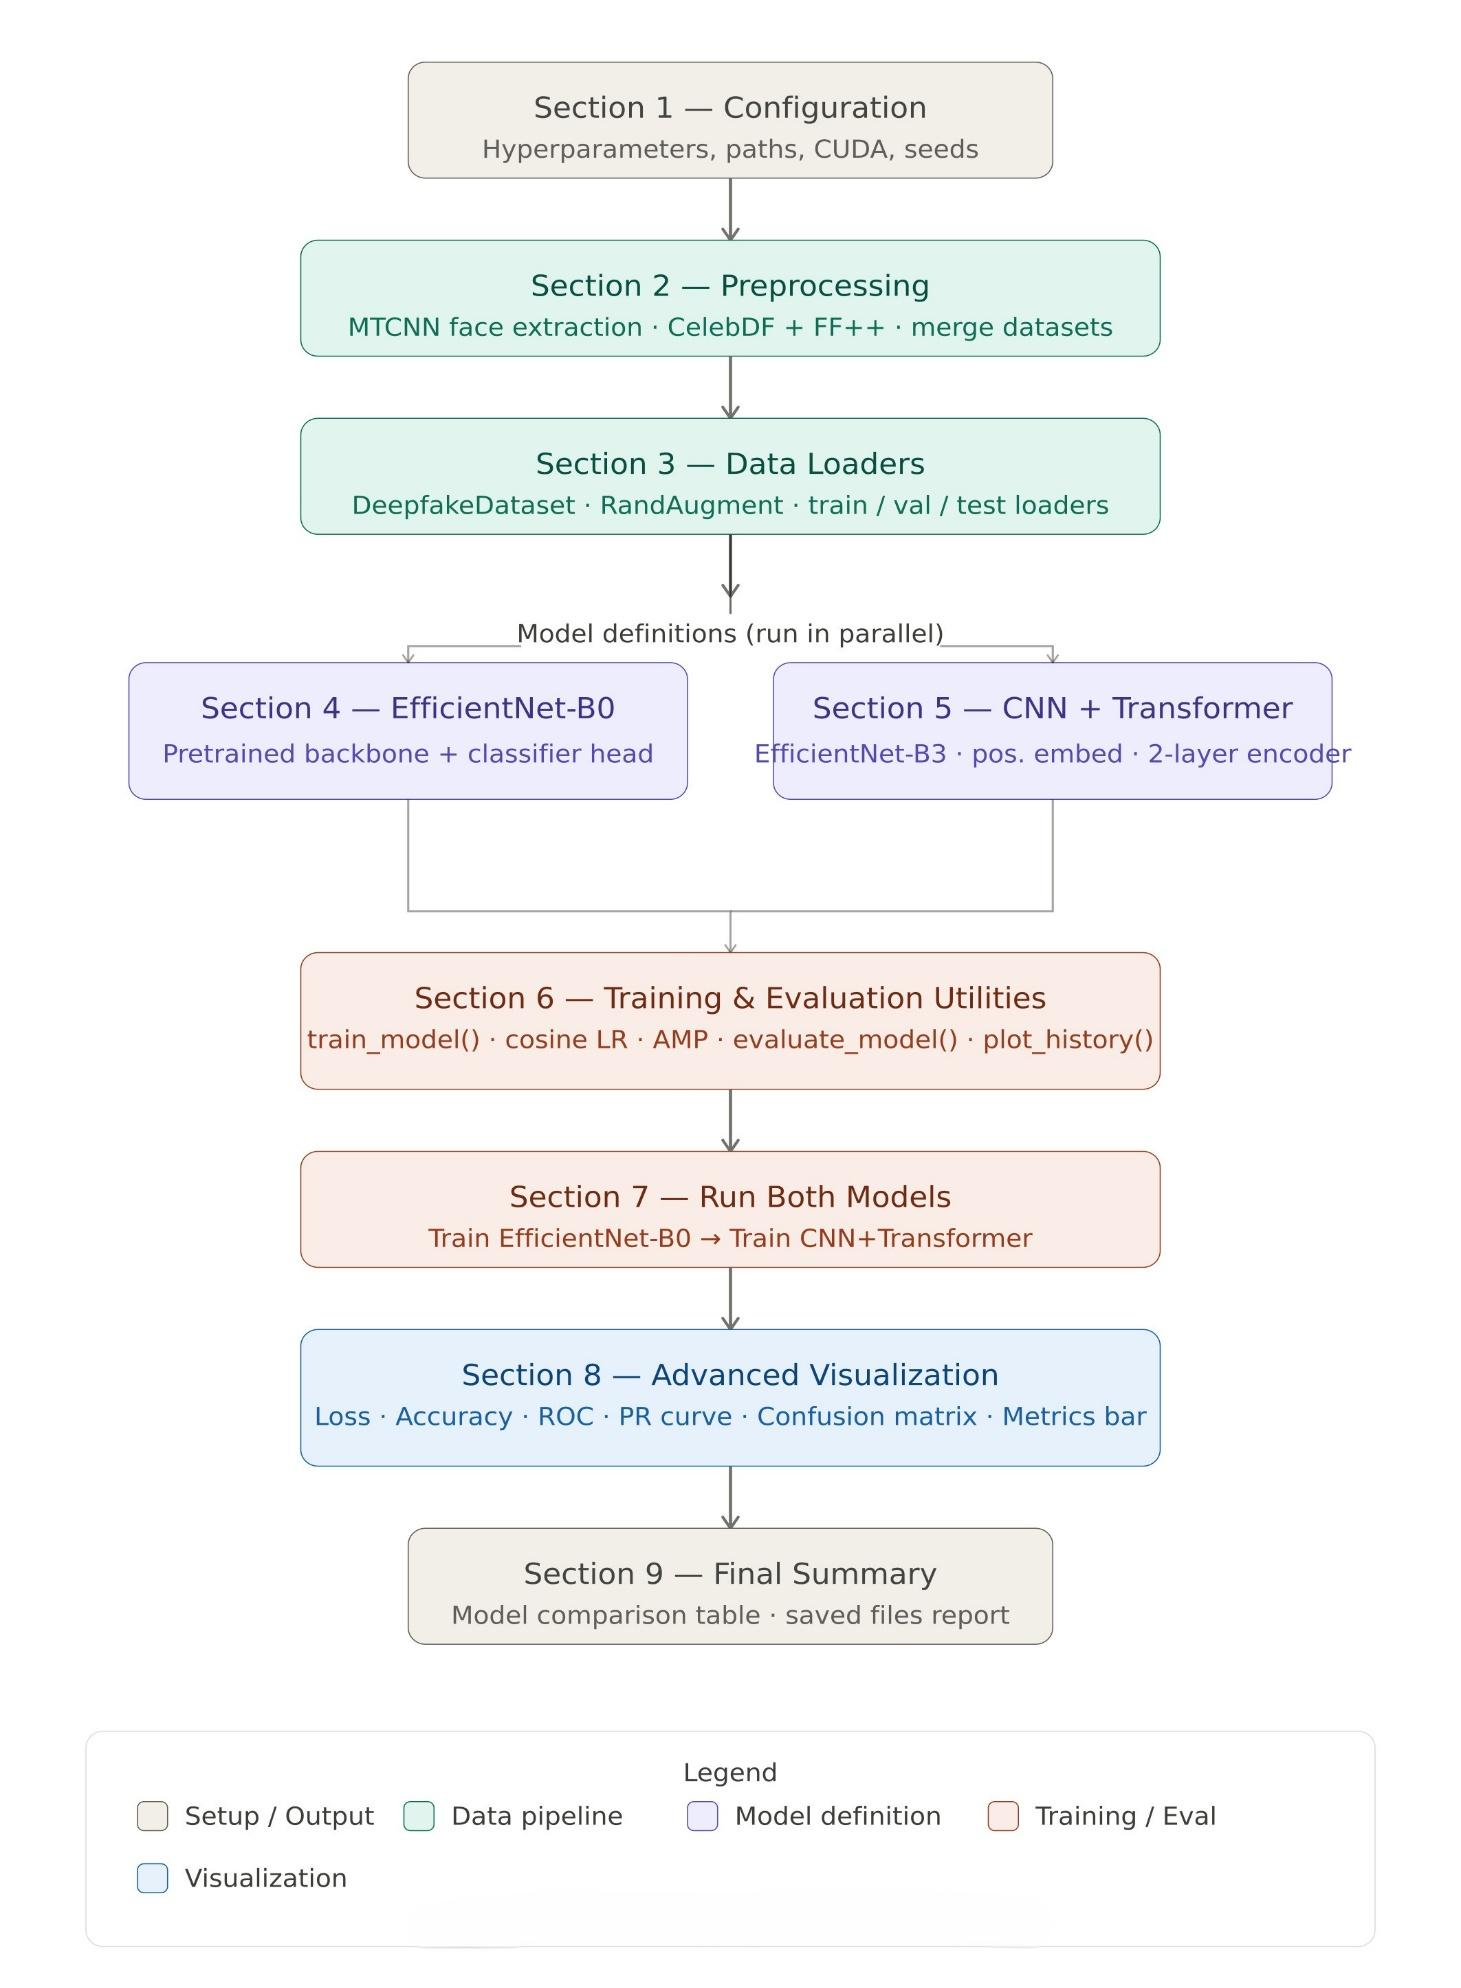
\includegraphics[width=0.8\textwidth]{11.png}
    \caption{}
    \label{fig:dataset_distribution}
\end{figure}

\addcontentsline{toc}{section}{Code Structure}



\newpage
\section*{Code Listings}
\addcontentsline{toc}{section}{Code Listings}

\begin{description}

\item[]

\par\noindent\textbf{Section 1 --- Configuration \& Speed Optimization}

\textbf{Title:} Global Hyperparameter Configuration and Hardware Setup

This section initializes all global hyperparameters and system-level settings required for the deepfake detection pipeline. It sets random seeds for reproducibility across Python, NumPy, and PyTorch, and configures dataset input/output directory paths for the CelebDF-V2 and FaceForensics++ (FF-C23) datasets. Key training parameters are defined here, including image size (224$\times$224), batch size (64), number of epochs (20), warmup epochs (3), and separate learning rates for the backbone (BACKBONE\_LR = 1e-5), transformer layers (TRANSFORMER\_LR = 5e-5), and classifier head (HEAD\_LR = 1e-4). Transformer architecture parameters such as embedding dimension (256), number of attention heads (4), encoder layers (2), feedforward dimension (512), and dropout (0.3) are also declared. The section detects GPU availability, enables cuDNN benchmark mode for speed, and initializes a mixed-precision GradScaler for automatic mixed precision (AMP) training.

\vspace{0.5cm}

\textbf{Section 2 --- Preprocessing Pipeline}

\textbf{Title:} Multi-Source Dataset Preprocessing with MTCNN Face Extraction

This section implements the complete data preparation pipeline for both video and image-based datasets. It uses the MTCNN (Multi-task Cascaded Convolutional Networks) face detector from facenet-pytorch to extract and align face regions from raw images and video frames. For the CelebDF-V2 dataset, frames are read from the pre-split train/val/test directories, resized to 320$\times$320, passed through MTCNN, and saved as 224$\times$224 face crops. For the FaceForensics++ dataset, video files from six manipulation categories (Deepfakes, Face2Face, FaceSwap, NeuralTextures, FaceShifter, DeepFakeDetection) and one authentic category (original) are sampled at every tenth frame, with up to ten face crops saved per video. A final merging function consolidates outputs from both datasets into a single unified combined\_data directory with standard train/val/test and real/fake folder structure.

\vspace{0.5cm}

\textbf{Section 3 --- Data Loaders}

\textbf{Title:} Dataset Construction with Augmentation Transforms and PyTorch DataLoaders

This section constructs the PyTorch Dataset and DataLoader objects used for training, validation, and testing. A custom DeepfakeDataset class is defined, which reads images from disk using PIL and applies configurable torchvision transforms. The training transform pipeline applies random horizontal flipping, random rotation ($\pm15^\circ$), colour jitter (brightness, contrast, saturation, hue), and RandAugment with two operations at magnitude 9 to improve generalisation, followed by normalisation using ImageNet mean and standard deviation values. The validation and test transforms apply only resizing and normalisation. Stratified train/validation splitting (80/20) is performed using scikit-learn, and class-balanced DataLoader objects are instantiated with configurable num\_workers and pin\_memory settings depending on device type.

\vspace{0.5cm}

\textbf{Section 4 --- Pretrained CNN Model (EfficientNet-B0)}

\textbf{Title:} EfficientNet-B0 Binary Classifier for Deepfake Detection

This section defines the first model architecture: a transfer-learning-based binary classifier built on EfficientNet-B0. The timm library is used to load a pretrained EfficientNet-B0 backbone with its classification head removed (num\_classes=0), yielding a 1280-dimensional feature vector per image. A custom classifier head is appended, consisting of a fully connected layer (1280$\rightarrow$512), ReLU activation, dropout (0.4), and a final linear layer (512$\rightarrow$2) for binary classification into real and fake classes. The model is transferred to the available compute device (GPU or CPU).

\vspace{0.5cm}

\textbf{Section 5 --- Hybrid CNN + Transformer Model}

\textbf{Title:} Hybrid EfficientNet-B3 and Transformer Encoder for Deepfake Detection

This section defines the primary proposed architecture: a hybrid model that combines a convolutional backbone with a Transformer encoder to capture both local texture features and global spatial relationships in face images. EfficientNet-B3 (pretrained via timm) serves as the backbone, producing spatial feature maps of shape (B, 1536, H, W). A LayerNorm is applied to the extracted features before projection to a 256-dimensional embedding space via a linear layer. The spatial dimensions are flattened into a sequence of patches, and learnable positional embeddings are added dynamically based on the actual spatial output size of the backbone (computed via a dummy forward pass to avoid hard-coded assumptions). A two-layer Transformer encoder with Pre-LayerNorm (norm\_first=True), four attention heads, 512-dimensional feedforward layers, and dropout of 0.3 processes the token sequence. Global average pooling is applied across the sequence dimension, and the resulting vector is passed through a three-layer classifier head (256$\rightarrow$128$\rightarrow$2) with GELU activations and dropout for final binary prediction.

\vspace{0.5cm}

\textbf{Section 6 --- Training \& Evaluation Utilities}

\textbf{Title:} Training Loop, Evaluation Metrics, and Visualization Utilities

This section provides the core training and evaluation infrastructure. Class-weighted cross-entropy loss with label smoothing (0.1) is computed from training set label frequencies to address class imbalance. The train\_model function implements a full epoch-based training loop with separate AdamW optimizer parameter groups, cosine annealing learning rate scheduling, automatic mixed precision (AMP), gradient clipping, and progressive backbone unfreezing. The best-performing model checkpoint is saved based on validation accuracy. The evaluate\_model function computes accuracy, precision, recall, and F1-score and plots a confusion matrix. The plot\_history function visualises training and validation accuracy and loss curves per epoch.

\vspace{0.5cm}

\textbf{Section 7 --- Model Training Execution}

\textbf{Title:} Sequential Training and Evaluation of Both Model Architectures

This section orchestrates the complete training pipeline by sequentially invoking the train\_model, evaluate\_model, and plot\_history functions for both the EfficientNet-B0 CNN model and the Hybrid CNN+Transformer model. Training histories, final predictions, and ground-truth labels are captured for each model and passed to the evaluation and visualization routines.

\vspace{0.5cm}

\textbf{Section 8 --- Advanced Graphs \& Visualization}

\textbf{Title:} Comprehensive Performance Visualization and Comparative Analysis

This section generates a suite of seven evaluation plots comparing the two trained models. These include training and validation loss curves, accuracy curves, validation accuracy comparisons, confusion matrices, ROC curves, precision-recall curves, and grouped metric comparison charts. All figures are saved to the designated graphs directory at 150 DPI.

\vspace{0.5cm}

\textbf{Section 9 --- Final Summary}

\textbf{Title:} Pipeline Summary and Saved File Report

This section consolidates the results of the complete training pipeline into a structured summary table. It records the best validation accuracy achieved by each model, the expected accuracy range, training speed, and GPU memory usage. The section also enumerates all generated artifact files, listing the graph images saved in the graphs directory and the model checkpoints saved in the checkpoints directory, confirming successful completion of the deepfake detection pipeline.

\end{description}
```



\end{document}